\chapter{Solar energy potential}
\label{solar}

\vspace{-45pt} % one line spacing corresponds approx to 15 pts
\begin{tcolorbox}[enhanced,width=\textwidth,size=fbox,
        sharp corners,colframe=black!5!white,drop fuzzy shadow southeast,
        boxrule=3mm, parbox=false] % other options: fontupper=\large\bfseries
This chapter is based on the article \citep{walch_big_2020}:

\qquad \bibentry{walch_big_2020}

and the conference proceedings \cite{walch_spatio-temporal_2019, walch_critical_2019, walch_fast_2019-1}:

\quad \bibentry{walch_spatio-temporal_2019} - \textit{Section~\ref{irrad}} 

\quad \bibentry{walch_critical_2019} - \textit{Section~\ref{solar_comparison}} 

\quad \bibentry{walch_fast_2019-1} - \textit{Section~\ref{solar_application}} 
\end{tcolorbox}

% SOURCE: Introduction ICAE paper
\begin{comment}
We use an Extreme Learning Machine (ELM) ensemble algorithm that allows to predict solar irradiance at an hourly time granularity for a high spatial resolution ($250 \times 250$) m$^2$ grid over Switzerland and to estimate the uncertainty related to the model and the data. The main advantages of this algorithm are (i) its fast training time and (ii) its ability to learn and to model complex non-linear phenomena with the desired precision. Hence this algorithm is well suitable for the analysis and modelling of large datasets [6,9,10].
\end{comment}

% SOURCE: PV Paper
The decarbonisation of the energy system plays an important role in fulfilling the ambitious emission targets set by the Paris Agreement \cite{peters_key_2017}. 
In this context, the large-scale deployment of rooftop-mounted photovoltaics (RPV) has attracted increasing attention in recent years \cite{jager-waldau_pv_2018}.
A quantitative assessment of the potential electricity generation from RPV is essential to formulate
%
effective incentive policies for their integration in the built environment. This requires accurate input data at a high spatial and temporal resolution in order to characterize regional differences and to assess the seasonal and intra-day variation of the generation \cite{bodis_high-resolution_2019}.
In addition, the analysis of RPV potential involves several uncertainties, which need to be quantified to facilitate interpretation of the results for policy making. 
 
Currently, there is no methodology that estimates the large-scale RPV potential at a high spatio-temporal resolution and also addresses the systematic propagation of uncertainties arising from the modelling process.
This paper contributes to fill this gap by adapting state of the art methods for the assessment of RPV potential in order to quantify and combine different sources of uncertainty. 
We further use Machine Learning to incorporate information that is only available in parts of the study region of Switzerland.

\begin{figure}[tb]
\centering\includegraphics[width=1.0\linewidth]{Figs/graphical_abstract_RPV.pdf}
\caption{Graphical abstract for the large-scale estimatio of hourly solar PV potential}
\label{fig:graphical_abstract_RPV}
\end{figure}

\section{Related literature}
% SOURCE: PV Paper
Constrained by the availability of building and environmental data at a high spatial resolution, most existing studies on RPV potential are carried out at district or city scale only, including case studies in the US \cite{levinson_solar_2009}, Canada \cite{nguyen_incorporating_2012}, Portugal~\cite{santos_applications_2014} or Germany \cite{strzalka_large_2012}. 
Few studies analyse an entire region or country, for example in the US \cite{phillips_data_2019, kodysh_methodology_2013}, Spain \cite{schallenberg-rodriguez_photovoltaic_2013}, or Saudia Arabia \cite{khan_rooftop_2017}. 
%
Many PV assessment studies use monthly or yearly solar radiation data in order to derive a large-scale PV potential \cite{ordonez_analysis_2010}. This data is used to quantify the available area to install PV \cite{mansouri_kouhestani_evaluating_2019} and to discuss the economic feasibility of PV scenarios \cite{romero_rodriguez_assessment_2017}.
While these granularities provide a relatively accurate estimation of the annual RPV potential, an hourly or higher temporal resolution is needed to assess the intra-day variation of the generation. Such temporal resolutions are used at the scale of cities or municipalities \cite{hong_development_2017, singh_estimation_2015} and serve to validate the estimations against measurements \cite{jakubiec_method_2013}, to compare PV technologies \cite{lukac_buildings_2014}, or to simulate energy systems with high shares of PV~\cite{wegertseder_combining_2016}. However, an hourly resolution is used very rarely at regional or national scale, in which case the available area to install PV is not addressed \cite{buffat_scalable_2018}.

Reasons for the lack of national-scale studies at an hourly temporal resolution are the computational challenges associated with the processing of the required input datasets as well as
the handling of missing data and data that is not available in the entire study region.
State of the art data processing techniques for estimating RPV potentials include physical models, geographic information systems (GIS), image processing and Machine Learning (ML). 
Physical models are used to compute the solar radiation on tilted surfaces, as well as the module and inverter efficiencies \cite{ramirez_camargo_spatio-temporal_2015}. 
GIS is applied to estimate shading effects and the sky view factor \cite{klauser_solarpotentialanalyse_2016, desthieux_solar_2018}.
The available area for installing PV is estimated in some studies using image recognition \cite{mainzer_assessment_2017, palmer_gis-based_2018}, while other methods use ML \cite{assouline_quantifying_2017, assouline_large-scale_2018}. 
These recent advances enable the integration of all mentioned aspects in high-resolution PV assessments at the national scale.
%
Missing data, in particular for predicting the available area for installing PV, is typically handled using constant coefficients and expert knowledge \cite{iea_potential_2002} or sampling techniques~\cite{wiginton_quantifying_2010}. Data with partial spatial coverage, i.e. information that is available only in parts of the study area, is successfully used in \cite{assouline_quantifying_2017, assouline_large-scale_2018} by applying ML. 
This method can be further improved by using different urban features and a larger training dataset.

To date, little research has quantified uncertainties for RPV potential assessments. Some studies address the uncertainties related to photovoltaic yield predictions for individual case studies \cite{thevenard_estimating_2013, gueymard_direct_2009}. In large-scale studies, confidence intervals are used in \cite{buffat_scalable_2018} to quantify the uncertainty related to the solar radiation, while they are used in \cite{assouline_large-scale_2018} to assess the available area for installing PV. 
The combination of different sources of uncertainty has been addressed through a scenario-based analysis for a local case study \cite{kreifels_uncertainty_2016} or by means of a sensitivity analysis \cite{martins_sensitivity_2016}. \citet{izquierdo_method_2008} provide a statistical propagation of uncertainty, which however focuses only on the available area for PV installation.
To the best of our knowledge, currently no methodology exists which quantifies and combines different sources of uncertainty related to the solar radiation and the available area that yields an uncertainty estimate on the technical RPV potential.

Our big data mining approach contributes to the existing literature by providing a methodology for a large-scale RPV potential and uncertainty estimation in hourly temporal resolution and a spatial resolution of individual roof surfaces. 
For this purpose, we combine state of the art physical models and GIS processing techniques with ML, 
which allows us to extract useful information from data that is only available in parts of the study area.
Our approach is used to quantify
(i) the spatio-temporal variation of the horizontal radiation, 
(ii) the effects of surrounding trees and buildings on roof shading and the sky view factor, 
(iii) the impact of roof geometry and roof superstructures, for example dormers and chimneys, on the available area for installing PV panels, 
and (iv) the temperature dependence of the PV module efficiency. 
We further present a systematic quantification of the uncertainties by treating each variable involved in the modelling process as a randomly distributed variable.
This allows to combine the uncertainties using their statistical distribution in order to obtain a total uncertainty on the technical potential estimate. 
The application of our method to 3.7 million buildings in Switzerland results in the first national-scale dataset of PV potential and uncertainty in hourly temporal resolution for individual rooftops. 

\begin{comment}
The paper is structured as follows. 
Section~\ref{data} introduces the datasets used in the study. 
Section~\ref{workflow_PV} describes the methodology for the computation of the RPV potential and the uncertainty propagation.
Section~\ref{solar_results} presents the results of the individual processing steps as well as the final technical RPV potential. A sensitivity analysis is performed to identify the most impactful steps of the estimation process.
Section~\ref{discussion_pv} discusses the methodological and practical contribution of the work and outlines its limitations and applications. 
Section~\ref{solar_conclusion} presents the conclusions and gives an outlook to future applications of the developed method.
\end{comment}

\begin{comment}
% SOURCE: Introduction ICAE paper
Current climate and environmental policies in Switzerland and worldwide aim at a strong reduction of CO$_{2}$ emissions in the next decades by transitioning from fossil fuels to renewable energy. Harvesting solar energy using photovoltaic (PV) and solar thermal technologies is one promising approach to achieve the ambitious emission targets. To determine the potential for large-scale deployment of solar technologies and to assess the requirements for a successful integration into the built environment, an accurate modelling of the spatial and temporal patterns of solar irradiance is essential. In this study, we present a methodology for modelling environmental variables at high spatial and temporal resolution by using large satellite datasets. We apply it to predict hourly global horizontal irradiance (GHI) on a ($250 \times 250$) m$^2$ grid, in order to be able to estimate PV potential at the neighborhood scale in Switzerland. 
Several data-driven methods exist to model solar irradiance. These include averaging the nearest neighbors [1], geostatistical methods such as kriging [2] as well as machine learning approaches such as Support Vector Machines [3], Random Forests [4] and neural networks [5,6]. As averaging tends to oversimplify the modelling, and kriging is computationally intensive and requires modelling of anisotropic spatial correlations and stationarity of the process, the data-driven machine learning algorithms have recently gained much attention due to their performance and speed [7]. Most studies however focus either on a high spatial or temporal resolution and frequently do not consider the uncertainty that is intrinsic to the modelling [8]. 

% SOURCE: Research plan
Several methods exist in the literature to map horizontal irradiance to obtain a physical solar energy potential. These include averaging the nearest neighbours [5], geostatistical methods such as kriging [18], [19] as well as machine learning approaches such as Support Vector Machines [3], Random Forests [20] and neural networks [21]–[23]. As averaging tends to oversimplify the modelling, and kriging is computationally intensive and requires modelling of anisotropic spatial correlations and stationarity of the process, the data-driven machine learning algorithms have recently gained much attention due to their performance and speed [24]. Most models do not estimate the uncertainty related to modelling horizontal irradiance, which is an important aspect if the results are processed further.
For an estimation of the geographic potential in urban environments, the most significant factors are shading effects and the determination of the area available for the installations [3]. Several methods exist to compute these in a detailed fashion, including image analysis and 3D modelling [25]. There are two main issues with computing urban factors for a large geographic area: 1) high-resolution datasets are typically not available everywhere, and 2) the computational time for exact methods is prohibitively high [7]. Different methods exist to approximate urban factors. These range from using standard tabulated factors based on expert opinions [26], statistical methods [7] and extrapolation techniques based on Machine Learning [3]. Assouline et al. [14] provide a detailed analysis of these methods. 
\end{comment}

\section{Methodology}
\label{solar_method}

\begin{figure}[tb]
\centering\includegraphics[width=1.0\linewidth]{Figs/solar_workflow.pdf}
\caption{Workflow for modelling of hourly solar PV potential. \textit{Input datasets }are described in Chapter~\ref{data}. \textit{Physical models} are provided in Chapter~\ref{phys_models}. \textit{Machine Learning} algorithms are summarised in Chapter~\ref{ML_supervised}. \textit{Geospatial (GIS) processing} methods are introduced in Chapter~\ref{GIS_methods}.}
\label{fig:workflow_PV}
\end{figure}

To estimate the RPV potential and its uncertainty, we propose a methodology that combines Machine Learning, GIS processing and physical models for the treatment of large spatio-temporal datasets, such as those presented in Chapter~\ref{data}.
Uncertainties are quantified from the statistical distribution of the variables involved in the potential estimation in the form of standard deviations.
They are assessed for various modelling steps and combined in order to obtain an uncertainty on the PV potential.

The method, illustrated in Fig. \ref{fig:workflow_PV}, is based entirely on open-source software and adopts an hierarchical approach used in several related studies \cite{izquierdo_method_2008, ramirez_camargo_spatio-temporal_2015, assouline_quantifying_2017}. Its steps include 
(i) the \textit{physical potential}, driven by the horizontal solar radiation, 
(ii) the \textit{geographic potential}, accounting for the impact of the built environment, and
(iii) the \textit{technical potential}, defined as the potential electricity generation.
The variables involved in each stage of the model and their relationships are explained below. The following subsections will detail the methodological contributions for the individual processing steps and the proposed quantification of uncertainty.

The physical potential is defined as the horizontal solar radiation at the earth's surface ($G_h$) for each time step $t$. The $G_h$ is composed of a direct beam component ($G_B$) and a diffuse component ($G_D$) such that \cite{loutzenhiser_empirical_2007}:

\begin{equation}
\label{eq:Gh}
G_{h}(t) = G_{B}(t) + G_{D}(t)
\end{equation}

The horizontal radiation is computed at a monthly-mean hourly (MMH) temporal resolution and a spatial resolution of $200 \times 200$ m$^2$, 
which is chosen as a trade-off between topographic detail and computational complexity as suggested in \cite{izquierdo_method_2008, assouline_large-scale_2018}. 
Each MMH time step represents an average value at a given hour of each month, across all days of the month. This leads to 288 distinct time steps, i.e. 24 hours for each of the 12 months. 
Using MMH values instead of 8760 hourly time steps allows to reduce the computational cost by a factor of 30, while preserving the daily and seasonal patterns of the average PV potential.
Any deviation from the MMH values is however covered by their uncertainty.

The geographic potential accounts for the rooftop geometry, for superstructures, for shading effects and for the sky visibility. It is estimated for each roof surface considering the tilted radiation ($G_t$) and the available roof area for PV panel installation ($A_{PV}$)  \cite{assouline_large-scale_2018}, such that:

\begin{equation}
\label{eq:irrad}
% G_{t}(t) = (1-S_{sh}(t)) * R_{B}(t)  G_{B}(t) + SVF * R_D(t)  G_{D}(t) + R_R(t)  G_h(t)
G_{t}(t) = (1-S_{sh}(t)) * G_{Bt}(t) + \mathit{SVF} * G_{Dt}(t) + G_{Rt}(t)
\end{equation}
\begin{equation}
\label{eq:area}
A_{PV} = A_{t} * C_{\mathit{pv}} * (1 - C_{sh})
\end{equation}

where $G_{Bt}$, $G_{Dt}$ and $G_{Rt}$ are direct, diffuse and reflected tilted radiation components, $\mathit{SVF}$ is the sky view factor, $A_{t}$ is the tilted roof area, $C_{\mathit{pv}}$ referred to as the \textit{panelled area coefficient} and $C_{sh}$ and $S_{sh}$ are referred to as the \textit{shaded area coefficient} and the \textit{hourly shading fraction} of the unshaded area, respectively.
%
The $C_{sh}$ represents the fraction of roof surface that is unshaded in less than 40\% of the daylight hours and is hence unsuitable for PV installation (see Section~\ref{shade}). The $S_{sh}(t)$ denotes the portion of the remaining roof area ($1 - C_{sh}$) that is shaded at each time step $t$. 
We treat $C_{sh}$ and $C_{\mathit{pv}}$, the proportion of roof area available to install PV panels, as independent factors. They are separately computed and it is assumed that no relevant overlap exists between the two factors. 
%
State of the art hourly physical models, described in Chapter~\ref{phys_models} (orange boxes in Fig.~\ref{fig:workflow_PV}), are used to obtain the tilted radiation components ($G_{Bt}, G_{Dt}, G_{Rt}$) 
We use the anisotropic Perez model \cite{perez_modeling_1990} to estimate $G_{Dt}$ , which is the overall most accurate diffuse radiation model \cite{noorian_evaluation_2008, loutzenhiser_empirical_2007}. 
The $G_{Rt}$ is computed using monthly mean albedo data (see Section~\ref{irrad}). This allows to account for snow cover in high-altitude locations, where a large albedo significantly increases the PV production on steep roofs~\cite{kahl_bright_2019}.

The technical potential ($E_{PV}$) is the electricity output of each roof surface. It is obtained from the geographic potential, the panel efficiency ($\eta_{PV}$) and the performance factor ($\mathit{PF}$), which accounts for inverter efficiency and other losses such as soiling or degradation, such that \cite{assouline_large-scale_2018}:

\begin{equation}
\label{eq:pv}
E_{PV} = G_t(t) * A_{PV} * \eta_{PV}(t) * \mathit{PF}(t)
\end{equation}
The module efficiency and performance factor are calculated for each time step $t$ from the tilted radiation and the ambient temperature using the \textit{PVWatts} model~\cite{dobos_pvwatts_2014} detailed in Chapter \ref{app:efficiency}. We use daily maximum temperature (see Table~\ref{tab:meteo}) to obtain a conservative estimate of the panel efficiency. 

Table \ref{tab:vars} summarizes the variables used above and the method applied to model each of them. 

\begin{table}[tb]
\centering
\footnotesize
\caption{Summary of the parameters used in the estimation of technical RPV potential. The dimension refers to $P$ for pixels of $200 \times 200$ m$^2$, $R$ for roof surfaces and $t$ for time steps. PM denotes the use of physical models.}
\label{tab:vars}
\begin{tabular} {lccccccc} % X[-1,c] X[-1,c] X[-1,c]
\hline 
  & $G_{h,B,D}$ & $G_{Bt,Dt,Rt}$ & $S_{sh}$   & $\mathit{SVF}$  & $C_{sh}$  & $C_{\mathit{pv}}$ & $\eta_{PV}, \mathit{PF}$     
  \\
\hline 
Dimension & $P \times t$ & $R \times t$ & $R \times t$ & $R$   & $R$     & $R$      & $R \times t$  
\\
Unit     & W/m$^2$    & W/m$^2$  & -                          & -                  & -                    & -                     & -                             
\\
Method      & ML & PM & GIS & GIS & GIS+ML & GIS+ML & PM \\
Section      & \ref{irrad}  & \ref{phys_models}     & \ref{shade}       & \ref{svf} & \ref{shade} & \ref{panels} & \ref{phys_models} 
\\  
\hline 
\end{tabular}
\end{table}

\begin{comment}
\subsection{Physical models}
\label{phys_models}

State of the art hourly physical models are used to (i) obtain the tilted radiation components ($G_{Bt}, G_{Dt}, G_{Rt}$) and (ii) to quantify the module and inverter efficiency. Both models, shown as orange boxes in Fig.~\ref{fig:workflow_PV}, are summarized in \ref{app:irrad}.
We use the anisotropic Perez model \cite{perez_modeling_1990} to estimate $G_{Dt}$ , which is the overall most accurate diffuse radiation model \cite{noorian_evaluation_2008, loutzenhiser_empirical_2007}. 
The $G_{Rt}$ is computed using monthly mean albedo data (see Section~\ref{irrad}). This allows to account for snow cover in high-altitude locations, where a large albedo significantly increases the PV production on steep roofs~\cite{kahl_bright_2019}.
The efficiencies are calculated for each time step $t$ from the tilted radiation and the ambient temperature using the \textit{PVWatts} model~\cite{dobos_pvwatts_2014}. We use daily maximum temperature (see Table~\ref{tab:meteo}) to obtain a conservative estimate of the panel efficiency. 


%%%%%%%%%%%%%%%%%%%%%%%%%%%%%%%%%%%%%%%%%%%%%%%%%%%%%%%

\subsection{Machine Learning}
\label{ML}

Machine Learning is used here  
(i) to obtain the horizontal radiation and the albedo at the $200 \times 200$ m$^2$ output grid from lower-resolution satellite data, 
(ii) to estimate the $C_{sh}$ and 
(iii) to account for the roof area covered by superstructures in the estimation of $C_{\mathit{pv}}$. 
We use supervised regression algorithms, which learn from a training set that contains pairs of inputs (features) and their known output values (targets). 
The models are then applied to predict unknown outputs for a new set of features.

We consider two ML algorithms, namely Random Forests (RF) \cite{breiman_random_2001} and Extreme Learning Machine Ensembles (ELM-E) \cite{huang_extreme_2006, wang_extreme_2015}. 
Both are ensemble algorithms which predict a target variable by averaging the results of multiple estimators (decision trees/ELMs) that have been trained on random re-samples of the training data \cite{breiman_bagging_1996}. 
Ensembles are well-suited for the estimaiton of uncertainties, which give a useful indication of the model's accuracy \cite{heskes_practical_1997}. 
%
The ELM-E is very efficient at modelling large datasets~\cite{de_freitas_viscondi_systematic_2019}, so we use this algorithm to estimate the hourly solar radiation and the monthly albedo. Preliminary work has shown that the RF outperforms the ELM-E for higher-dimensional datasets with less training data. The RF is hence used to estimate $C_{sh}$ and $C_{\mathit{pv}}$.

To optimize the performance of each ML model, it is necessary to firstly select its features, and secondly to choose the parameters defining the structure of each model through hyper-parameter tuning. 
In the following sections, we will focus on the feature selection and the performance of the optimized ML models. Information regarding the tuning of the algorithms is provided in \ref{app:tuning}.

%%%%%%%%%%%%%%%%%%%%%%%%%%%%%%%%%%%%%%%%%%%%%%%%%%%%%%%
\end{comment}

\subsection{Horizontal solar radiation and albedo}
\label{irrad}

We propose an ML-based approach to estimate the horizontal radiation and the surface albedo for pixel maps of $200 \times 200$ m$^2$ resolution, as presented in the blue box in Fig.~\ref{fig:workflow_PV}-A.
The ML models yield the global ($G_h$) and direct ($G_B$) horizontal radiation for each MMH time step $t$ and the albedo ($\rho$) as monthly mean values. 
The diffuse radiation ($G_D$) is obtained from the estimated $G_h$ and $G_B$ by applying Eq.~(\ref{eq:Gh}). 
Using ML, we can model complex spatial patterns while being more efficient than other spatial interpolation methods such as kriging~\cite{rehman_spatial_2000}. 

The targets for the ML models of $G_h$ and $G_B$ are the satellite-derived global and direct radiation, which are split into 12 monthly subsets (see Chapter~\ref{data_meteo}).
The initially considered set of features are the mean hour of each month, the geographic coordinates (x, y) as well as several terrain features including altitude (z), terrain slope and curvature \cite{robert_spatial_2012} (see Chapter~\ref{data_DEM} for details). 
A DTM is used to derive these terrain features for the satellite data and for the $200 \times 200$ m$^2$ output grid. 
To better model the spatio-temporal patterns of $G_h$ and $G_B$, we analyze the spatial features for each time step using the RF feature importance score~\cite{pedregosa_scikit-learn:_2011}.
Figure \ref{fig:ftrs_phys} shows their pattern for the months of June and December.
The feature importance exhibits a strong intra-day variation for x, y and z, which may be explained by the impact of the Swiss alpine terrain. All other features have an overall low importance throughout the day, and including these in the model does not improve its performance further.
Four features are hence selected for the final model: hour, x, y, z.
Figure \ref{fig:ftrs_phys} refers to $G_h$, but $G_B$ shows a similar trend.

Separate ELM-E are trained for each month for $G_h$ and $G_B$. For model training, the $G_h$ and $G_B$ for 80\% of the 11,243 satellite pixels ($\approx 9,000$) are used for training, while the rest are kept for the test set. Their tuning procedure and the resulting hyper-parameter values of the models are provided in Appendix \ref{app:tune_ELM}. 
Table \ref{tab:G_train} shows the mean-squared error (MSE) between the targets and predictions for the test set, while Fig.~ \ref{figc:ELM_training} shows the fit of the predictions and the targets ($G_h$ only). Each entry (color) represents one trained monthly ELM-E.
The model performance is overall better for $G_h$ than for $G_B$, as it is harder to model $G_B$ from the given set of features.
%
To estimate $\rho$ from the satellite-derived daily albedo measurements, we train one ELM-E with similar features as described above, namely x, y, z and month. The model is tuned in a similar fashion as that of $G_h$ and $G_B$ and yields a test MSE of 0.10, which lies in the range of the values obtained for $G_h$.

\begin{figure}[tb]
\centering
\begin{subfigure}{.32\textwidth}
  \centering
  % include second image
  \includegraphics[width=\linewidth]{Figs/importance_July.pdf}  
\end{subfigure}
\begin{subfigure}{.32\textwidth}
  \centering
  % include first image
  \includegraphics[width=\linewidth]{Figs/importance_December.pdf}  
\end{subfigure}
\begin{subfigure}{.32\textwidth}
  \centering
  % include second image
  \includegraphics[width=\linewidth]{Figs/corr_test_data.pdf}  
  \caption{}
  \label{figc:ELM_training}
\end{subfigure}
\caption{Feature importance per hour for $G_h$ for June (a) and December (b) for six terrain features, namely altitude (z), longitude (x), latitude (y), medium-scale curvature (medDoG), small-scale curvature (smallDoG), terrain slope in east-west (big\_EW) and north-south (big\_NS) direction. (c) Fit of predictions and targets for $G_h$ per month (test set) and the linear regression curve (black line) fitted on targets and predicted values.}
\label{fig:ftrs_phys}
\end{figure}

\begin{table}[tb]
\centering
\footnotesize
\caption{Test mean-squared error (MSE) for the estimation of $G_h$ and $G_B$.}
\label{tab:G_train}
\begin{tabular}{lcccccccccccc}
\hline 
 \textbf{MSE}   & Jan  & Feb  & Mar   & Apr   & May   & Jun   & Jul   & Aug   & Sep   & Oct  & Nov  & Dec  \\
\hline 
$G_h$  & 0.10 & 0.07 & 0.07  & 0.06  & 0.06  & 0.04  & 0.06  & 0.05  & 0.12  & 0.10 & 0.10 & 0.06 \\
$G_B$  & 0.17 & 0.12 & 0.18 & 0.17 & 0.21 & 0.14  & 0.18  & 0.12 & 0.26 & 0.16 & 0.21 & 0.11 \\
\hline 
\end{tabular}
\end{table}

%%%%%%%%%%%%%%%%%%%%%%%%%%%%%%%%%%%%%%%%%%%%%%%%%%%%%%%%%%%%%%%%%

\subsection{Available area for PV panel installation}
\label{panels}

The \textit{panelled area coefficient} $C_{\mathit{pv}}$ describes the available roof area for PV installation considering the roof geometry and superstructures. To compute $C_{\mathit{pv}}$, we use a geospatial algorithm in combination with ML, as represented by the green and blue box yielding $C_{\mathit{pv}}$ in Fig.~\ref{fig:workflow_PV}-B.
%
The geospatial algorithm, detailed in \ref{app:virtualPV}, virtually installs PV panels by projecting rectangular polygons onto the tilted roofs as shown in Fig.~\ref{fig:panels}. The $C_{\mathit{pv}}$ is then obtained from the number of installed panels.
The panels are installed in both horizontal and vertical alignments, as no alignment has technical advantages over the other and both are widespread. The configuration with a higher number of panels is selected for each roof.

\begin{figure}[tb]
\centering
\begin{subfigure}{.5\textwidth}
  \centering
  % include first image
  \includegraphics[width=.8\linewidth]{Figs/panels3.pdf}  
\end{subfigure}
\caption{Output of the virtual installation of PV panels after removing roof superstructures. The best configuration of vertically and horizontally oriented panels is selected. Panels on flat roofs are placed in south-facing rows and tilted at an optimal angle of 30$^\circ$.}
\label{fig:panels}
\end{figure}

The data on roof superstructures is however only available in one of Switzerland's 26 cantons (Geneva). We hence train an ML model to estimate the change in $C_{\mathit{pv}}$ due to the area covered by superstructures, which is applied to the rooftops of the remaining 25 cantons. 
%
In our case, the training of the ML model is performed using the rooftop dataset with superstructure information in the Canton of Geneva (see Section~\ref{data}).
The fraction of their area on which virtual panels are installed provides the target for the ML algorithm ($C_{\mathit{pv}}^T$).
In addition, we define $C_{\mathit{pv}}^F$ as the fraction of the area on which virtual panels can be installed if no superstructures are removed from the roof polygons. This $C_{\mathit{pv}}^F$ is one feature of the ML model. %
The full set of the considered features is listed in Table \ref{tab:features}. 
Figure~\ref{fig:RF_Cpv} shows the feature importance for all inputs. 
While the top six features have the highest importance, 
the complete set of features is used for modelling $C_{\mathit{pv}}$ as this has been found to improve the estimation precision.

\begin{table}[b]
\centering
\footnotesize
\caption{Features considered in the ML models to estimate $C_{\mathit{pv}}$ and $C_{sh}$. $^1$The building density is computed as the number of building coordinates within a 100 m radius of each roof. $^2$The roof perimeter, shape index (perimeter per area) and vertex count are derived from the polygon data.}
\label{tab:features}
\begin{tabular}{lll}
\hline
\textbf{Computed features}               & \textbf{Roof features} & \textbf{Building features} \\
\hline
$C_{\mathit{pv}}^F$ / $C_{sh}^F$ & Tilted area                          & Footprint area                              \\
Panel tilt   & Tilt angle                          & Building type                              \\
(not used for $C_{sh}$)      & Aspect angle                        & Construction period          \\
Build. density$^1$                    & Perimeter$^2$                       & Number of floors                             \\
                                 & Shape index$^2$                       &   \\
 & Vertex count$^2$ & \\ 
\hline                                
\end{tabular}
\end{table}

Table~\ref{tab:errors_Cpv} reports the residuals between $C_{\mathit{pv}}^F$ and $C_{\mathit{pv}}^T$ (baseline), as well as the cross-validation error between the estimated $C_{\mathit{pv}}$ and the target $C_{\mathit{pv}}^T$ in the case of additive bias correction (MBE+) and for using the tuned RF model (see \ref{app:tune_RF} for details).
The bias correction is performed by adding the mean bias error (MBE) between $C_{\mathit{pv}}^F$ and $C_{\mathit{pv}}^T$  to all samples. 
We compare the root mean squared error (RMSE), mean absolute error (MAE), MBE and the R$^2$ coefficient of determination. All methods remove the negative baseline bias of 17\%. The RF outperforms the bias correction, as it achieves lower errors and a higher R$^2$. It is hence used to estimate the $C_{\mathit{pv}}$ used in Eq.~(\ref{eq:area}).

\begin{figure}[tb]
\centering
  \includegraphics[width=.5\linewidth]{Figs/Feature_importance_panels.pdf}
\caption{Feature importance of all features considered for the estimation of $C_{\mathit{pv}}$.
}
\label{fig:RF_Cpv}
\end{figure}

\begin{table}[tb]
\centering
\footnotesize
\caption{Errors for estimating $C_{\mathit{pv}}$. We compare the residuals between $C_{\mathit{pv}}^F$ and $C_{\mathit{pv}}^T$ (baseline) with the cross-validation error between the estimated $C_{\mathit{pv}}$ and the target $C_{\mathit{pv}}^T$ in the case of bias correction (MBE+) and for using the Random Forest model (RF).}
\label{tab:errors_Cpv}
\begin{tabular}{lcccc}
\hline
      & \textbf{Baseline} & \textbf{MBE+}  & \textbf{RF}   \\ \hline
RMSE  & 0.23     & 0.15  & 0.12 \\
MAE   & 0.17     & 0.12  & 0.09 \\
MBE   & -0.17    & 0.00  & 0.00 \\
R$^2$ & -0.10    & 0.52  & 0.69 \\ \hline
\end{tabular}
\end{table}

%%%%%%%%%%%%%%%%%%%%%%%%%%%%%%%%%%%%%%%%%%%%%%%%%%%%%%%%%%%%%%%%%%%%%%%%%

\subsection{Shading effects and sky view factor}
\label{shade}
\label{svf}

To quantify shading effects from surrounding buildings and trees, we use a shadow casting approach \cite{buffat_scalable_2018, desthieux_solar_2018, klauser_solarpotentialanalyse_2016, ramirez_camargo_spatio-temporal_2015}. 
In contrast to the existing studies, we account for the shading effects in two ways:
First, strong shading effects may render parts of a roof unsuitable for installing PV. 
Second, some of the suitable area may be shaded at particular hours and reduce the PV potential for these hours. We hence distinguish between the \textit{shaded area coefficient} ($C_{sh}$), the fraction of roof area which is unsuitable due to shading, and the \textit{hourly shading fraction} ($S_{sh}(t)$), which is computed for each hour as the shaded portion of the remaining roof. 

The shadow casting approach (green box in Fig.~\ref{fig:workflow_PV}-B) models shadows on building roofs for each pixel of a DSM at a given sun position. It is used to produce hourly shadow maps for the representative day of each month (close to day 15~\cite{desthieux_solar_2018}) and hence yields results at the same temporal resolution as the solar radiation.
Figure~\ref{fig:horizons}a shows an example of these maps. They are binary maps, with a 0 (dark areas) representing a cast shadow and a 1 (yellow areas) indicating direct sun exposure. The shadow maps are averaged for all daylight hours, resulting in the mean illumination map shown in Fig.~\ref{fig:horizons}b. Its values represent the percentage of time steps for which each pixel is unshaded.

All areas with a mean illumination lower than the average value across all roofs (red areas) are considered unsuitable. 
We compute this average value as 42.7\% and hence use a rounded threshold of 40\% mean illumination to exclude unsuitable areas.
Dividing the red areas in Fig.~\ref{fig:horizons}b by the total roof area yields $C_{sh}$, while $S_{sh}$ is the fraction of zeros in Fig.~\ref{fig:horizons}a on the suitable (non-red) surfaces at time $t$. The GIS algorithm for shading effects is given in \ref{app:shade}. 

\begin{figure}[tb]
	\centering
	\begin{subfigure}{.52\textwidth}
		\centering
		% include first image
		\includegraphics[trim=25 0 10 0, clip, width=.8\linewidth]{Figs/3d_shade.pdf} 
		\subcaption{}
	\end{subfigure}
	\begin{subfigure}{.44\textwidth}
		\centering
		% include first image
		\includegraphics[width=.8\linewidth]{Figs/shade_mean.pdf}  
		\subcaption{}
	\end{subfigure}
	\caption{a) binary shadow maps used to derive $S_{sh}$, for 5 example time steps (0: cast shadow, 1: sun exposure). b) mean illumination map used to compute $C_{sh}$ (red areas).}
	\label{fig:horizons}
\end{figure}

Two datasets are available to compute $C_{sh}$ and $S_{sh}$: the national DSM$_{2\text{m}}$ and the DSM$_{50\text{cm}}$ for the canton of Geneva (see Table~\ref{tab:bld_landscape}). Our method aims at enhancing the national-scale $C_{sh}$ and $S_{sh}$ from the DSM$_{2\text{m}}$ based on knowledge extracted from the DSM$_{50\text{cm}}$, which is more recent and detailed. For this task, we denote the values extracted from the DSM$_{2\text{m}}$ as $C_{sh}^F$, $S_{sh}^F$ (features) and those obtained from the DSM$_{50\text{cm}}$ as $C_{sh}^T$, $S_{sh}^T$ (targets).
%
Their comparison yields an MBE of 2.7\% between $S_{sh}^F$ and $S_{sh}^T$ and of 8.9\% between $C_{sh}^F$ and $C_{sh}^T$. As the MBE for $S_{sh}$ is small compared to the order of magnitude of other uncertainties, we use an additive bias correction (MBE+) to correct $S_{sh}^F$ at the national scale, applied separately for each time step. 

The $C_{sh}$ shows a larger bias, so $C_{sh}^F$ systematically underestimates the shaded area coefficient. This leads to an overestimation of available area. 
As a mean bias correction (MBE+) increases the MAE (see Table~\ref{tab:errors_Csh}), we apply an ML model (RF) to estimate $C_{sh}$, illustrated by the blue box yielding $C_{sh}$ in Fig.~\ref{fig:workflow_PV}-B. 
The features that are used to estimate  $C_{sh}$ are listed in Table~\ref{tab:features}.
Figure~\ref{fig:RF_Csh} shows the feature importance for $C_{sh}$. Interestingly, the building type has a high importance. This may be due to the different objects that cause shading on buildings. 

The errors for estimating $C_{sh}$ are shown in Table~\ref{tab:errors_Csh}. While the improvement of the MAE when using ML is relatively small, we do observe a large improvement in the R$^2$ coefficient.
Unpredictable factors, such as discrepancies between the DSM$_{2\text{m}}$ and the DSM$_{50\text{cm}}$ or mismatches between the roof polygons and the DSMs, keep even the improved R$^2$ coefficient rather low. 
These errors will be reflected in the results by an increased uncertainty.

\begin{figure}[tb]
\centering
\includegraphics[width=.5\linewidth]{Figs/Feature_importance_shade.pdf}  
\caption{Feature importance of all features considered for the estimation of $C_{sh}$.}
\label{fig:RF_Csh}
\end{figure}

\begin{table}[tb]
\centering
\footnotesize
\caption{Errors for estimating $C_{sh}$. Baseline is the error between $C_{sh}^F$ and $C_{sh}^T$, for MBE+ and RF models.}
\label{tab:errors_Csh}
\begin{tabular}{lcccc}
\hline
      & \textbf{Baseline} & \textbf{MBE+} & \textbf{RF}   \\ \hline
RMSE  & 0.23     & 0.21  & 0.18 \\
MAE   & 0.13     & 0.14  & 0.12 \\
MBE   & 0.09     & 0.00  & 0.00 \\
R$^2$ & 0.12     & 0.25  & 0.44 \\ \hline
\end{tabular}
\end{table}

The sky view factor (SVF), representing the visible proportion of the sky, is computed by combining the vertical elevation angles of the horizon for a discretized set of directions \cite{zaksek_sky-view_2011}. We find 32 equally spaced directions to be sufficient for a precise estimation of the SVF, which we have implemented according to \ref{app:shade}.
Using the DSM$_{2\text{m}}$ and the DSM$_{50\text{cm}}$, we compute a national $\mathit{SVF}^F$ and a "true" $\mathit{SVF}^T$ in Geneva, respectively. The MBE between the two variables is 7.16\%.  
As the error of $\mathit{SVF}^F$ with respect to $\mathit{SVF}^T$ follows no identifiable pattern given the available features, we apply bias-correction (MBE+) to adjust the $\mathit{SVF}^F$ at national scale based on data from the high-resolution DSM$_{50\text{cm}}$, similar to $S_{sh}$ in Section~\ref{shade}.

%%%%%%%%%%%%%%%%%%%%%%%%%%%%%%%%%%%%%%%%%%%%%%

\subsection{Flat rooftops}
\label{flat}

For a more realistic representation of PV panels on flat roofs, we assume PV panels to be installed in individual south-facing rows instead of placing them in consecutive rows along the roof aspect. Some spacing is left between the rows to reduce mutual shading effects between them (see Fig~\ref{fig:panels}).
The tilt angle and row spacing is chosen as a trade-off between the total PV output and the capacity factor, which is a proxy of the economic feasibility.
We have simulated different configurations and found a technically optimal trade-off for a tilt angle of $30^\circ$ and a spacing of one panel height at the Swiss latitude.

The installation strategy on flat roofs impacts the PV potential in multiple ways: (i) tilted radiation increases due to the panel tilt of $30^\circ$, (ii) $C_{\mathit{pv}}$ decreases due to the spacing of the rows, (iii) mutual shading between adjacent rows of panels increases the hourly shaded fraction and (iv) the sky view factor is reduced. The $S_{sh}$ and the $\mathit{SVF}$ of flat roofs are hence multiplied with an additional hourly shading factor ($S_{\mathit{flat}}(t)$) and sky view factor ($\mathit{SVF}_{\mathit{flat}}$), respectively, which we have simulated using the geometric model explained in Chapter~\ref{app_flat}. 

%%%%%%%%%%%%%%%%%%%%%%%%%%%%%%%%%%%%%%%%%%%%%%%%%%%%%%%

\subsection{Uncertainty}
\label{unc}

The technical potential depends on multiple variables, as shown in Fig.~\ref{fig:workflow_PV}. 
The best estimate for each variable is given by their first and second order moments, which may be used to combine various uncertainties using statistical methods.
%
Uncertainties arise from different sources and are unknown in some cases. 
In this work, we consider only those uncertainties for which information can be extracted from the statistical analysis of our data. Further potential sources of uncertainty will be discussed in Section~\ref{limitations_pv}.

\subsubsection{Uncertainty for ML methods}

To estimate the uncertainties for the output variables of the ML models, namely $G_h, G_B, \rho, C_{sh}$ and $C_{\mathit{pv}}$, we follow the two-stage approach presented in Chapter~\ref{unc_ML}. 
It distinguishes between the uncertainty arising from the modelling process (model uncertainty, $\sigma_M$) and the uncertainty related to the data noise (data uncertainty, $\sigma_D$) \cite{wan_probabilistic_2014}. 
The data uncertainty may also represent errors introduced by previous processing steps, for example using GIS. 

The model uncertainty is estimated as the standard deviation of the predictions from each ensemble member of the RF or ELM-E \cite{heskes_practical_1997, wan_probabilistic_2014}. 
To quantify the data uncertainty, a second ML model is trained on the remaining residuals of the out-of-bag training data~\cite{breiman_bagging_1996}, which are derived from the squared difference between the targets and predictions~\cite{heskes_practical_1997, wan_probabilistic_2014}. This second ML model is used to predict $\sigma_D$ for each predicted output (see Chapter~\ref{unc_ML} for details). In this work, we use the same hyper-parameters for the residual model as we use for the respective primary ML model (i.e. $G_h, G_B, \rho, C_{sh}$ and $C_{\mathit{pv}}$), reported in Appendix \ref{app:tuning}.
% Further information regarding our implementation of this method is provided in Chapter~\ref{unc_ML}.
The total uncertainty of a variable estimated using ML is then the squared sum of its model uncertainty and its data uncertainty.

% SOURCE: ELM PAPER
\begin{comment}
The observed spread represents the intrinsic data uncertainty which we measure using the residuals. For modelling these residuals, an analysis equivalent to the one presented above is conducted, giving optimal model hyper-parameters of L = 500 and M = 50.
\end{comment}

\subsubsection{Uncertainty for GIS methods}

The uncertainty for the GIS-derived and bias corrected quantities ($S_{sh}$ and $\mathit{SVF}$) is estimated from the residuals between the values computed using the national DSM$_{2\text{m}}$ ($S_{sh}^F$, $\mathit{SVF}^F$) and the "true" values extracted from the DSM$_{50\text{cm}}$ ($S_{sh}^T$, $\mathit{SVF}^T$) in Geneva.
The error is treated as a random variable, whose first and second moments are computed as the mean and the variance of these residuals. The mean is used for the bias correction, as explained in Sections \ref{shade} and \ref{svf}, while the variance represents the uncertainty.

\subsubsection{Uncertainty propagation}
\label{unc_prop}

The propagation of uncertainty is performed by treating Eqs.~(\ref{eq:Gh})-(\ref{eq:pv}) as functions of randomly distributed variables with statistical errors. 
To compute the variances of their output variables from a combination of the means, variances and covariances of their inputs (summarized in Table~\ref{tab:vars}), we make the following assumptions:
First, statistical independence is assumed between the solar radiation ($G_{h, B, D}$) and the DSM-derived variables ($S_{sh}, \mathit{SVF}$). 
This is valid as the uncertainty of $G_{h, B, D}$ is dominated by the meteorological variability, while that of $S_{sh}(t)$ and $\mathit{SVF}$ is related to errors in the GIS methods. These are independent and uncorrelated processes. 
By contrast, $G_h$ and $G_B$, as well as $S_{sh}$ and $\mathit{SVF}$, exhibit a mutual correlation, as Table~\ref{tab:covrr} shows. Therefore, their covariances must be considered in the uncertainty propagation. 
Second, we assume that $G_t$ and $A_{PV}$, and $C_{\mathit{pv}}$ and $C_{sh}$, are independent as their correlation coefficients are negligible (see Table~\ref{tab:covrr}).
Third, we neglect the uncertainties of $\rho$ and of the temperature data, as these have a low impact on the final results.
Fourth, we do not account for the uncertainty related to the physical models of $G_{Dt}$, $\eta_{PV}$ and $\mathit{PF}$ (Section~\ref{phys_models}), due to a lack of data on their performance and the expected errors. This limitation will be discussed in Section \ref{limitations_pv}.

\begin{table}[tb]
\centering
\footnotesize
\caption{Linear correlation coefficients for pairs of potentially correlated random variables. $^1$ denotes a spatio-temporal mean, $^2$ indicates a mean across all time steps $t$.}
\label{tab:covrr}
\begin{tabular}{lc}
    \hline
                        & \textbf{Correlation}  \\ \hline
    $G_h$, $G_B$ $^1$    & 0.87                  \\
    $S_{sh}$, $\mathit{SVF}$ $^2$  & 0.36                  \\ 
    $G_t$, $A_{PV}$ $^2$  & 0.04                  \\
    $C_{\mathit{pv}}$, $C_{sh}$    & 0.02                  \\   \hline 
\end{tabular}
\end{table}

Table~\ref{tab:uncs} summarizes all variables for which uncertainties are considered, as well as the dimensions along which these are derived.
Based on the above assumptions and given the uncertainties in Table~\ref{tab:uncs}, the variances of $G_D$ ($\sigma^2_{GD}$) and $G_t$ ($\sigma^2_{Gt}$) are derived from Eqs.~(\ref{eq:Gh}) and (\ref{eq:irrad}) using the error propagation theory summarized in Chapter~\ref{method_unc_prop}, such that:

\begin{equation}
\label{eq:unc_GD}
\sigma^2_{GD} = \sigma^2_{Gh} +  \sigma^2_{GB} - 2 \mathrm{Cov}(G_h, G_B) 
\end{equation}
%
\begin{equation}
\label{eq:irrad_unc}
\sigma^2_{Gt} = \sigma^2_{B} +  \sigma^2_{D} +  \sigma^2_{R} + 2 (\mathrm{Cov}(B, D) + \mathrm{Cov}(B, R) + \mathrm{Cov}(D, R))
\end{equation}

where the direct, diffuse and reflected components of $G_t$ are denoted as $B=(1 - S_{sh}) * G_{Bt}$, $D=\mathit{SVF} * G_{Dt}$ and $R=G_{Rt}$. The expressions for their variances ($\sigma^2_{B}, \sigma^2_{D}, \sigma^2_{R}$) and covariances are provided in \ref{unc_Gt}. 

The variances of $A_{PV}$ ($\sigma^2_A$) and $E_{PV}$ ($\sigma^2_{PV}$) are derived from Eqs.~(\ref{eq:area}) and (\ref{eq:pv}), respectively:

\begin{equation}
\label{eq:area_unc}
% Definition of variance of diffuse component     
\sigma^2_{A}  = A_{t}^2 (\sigma^2_{\mathit{Csh}} C_{\mathit{pv}}^2 + \sigma^2_{\mathit{Cpv}} (1-C_{sh})^2 + \sigma^2_{\mathit{Csh}} \sigma^2_{\mathit{Cpv}}) 
\end{equation}
%
\begin{equation}
\label{eq:pv_unc}
% Definition of variance of diffuse component     
\sigma^2_{PV}  = \eta_{PV}^2 \mathit{PF}^2 (\sigma^2_{A} G_{t}^2 + \sigma^2_{Gt} A_{PV}^2 + \sigma^2_{Gt} \sigma^2_{A}) 
\end{equation}

\begin{table}[tb]
\centering
\footnotesize
\caption{Summary of the uncertainties for each variable in the RPV potential estimation. The dimension (dim) of the uncertainties refers to $R$ as roof surfaces and $t$ as time steps.}
\label{tab:uncs}
\begin{tabular} {lcccccccc}
\hline 
\textit{Variable}  & $G_{h,B,D}$  & $S_{sh}$  & $\mathit{SVF}$ & $C_{sh}$ & $C_{\mathit{pv}}$ & $G_t$  & $A_{PV}$ & $E_{PV}$                  \\
\hline 
Uncertainty    & $\sigma_{Gh,B,D}$    & $\sigma_{\mathit{Ssh}}$     & $\sigma_{\mathit{SVF}}$     & $\sigma_{\mathit{Csh}}$  & $\sigma_{\mathit{Cpv}}$    & $\sigma_{Gt}$   & $\sigma_{A}$     & $\sigma_{PV}$                     \\
Dim. of $\sigma$ & $R \times t$ & $t$ & $1$   & $R$     & $R$     & $R \times t$ & $R$    & $R \times t$ \\
\hline 
\end{tabular}
\end{table}

%%%%%%%%%%%%%%%%%%%%%%%%%%%%%%%%%%%%%%%%%%%%%%%%%%%%%%%
%%%%%%%%%%%%%%%%%%%%%%%%%%%%%%%%%%%%%%%%%%%%%%%%%%%%%%%

\begin{comment}

\subsection{Prediction and uncertainties}

After defining the model parameters and training the model on the satellite data, we predict the monthly-mean-hourly GHI on a dense grid over Switzerland and estimate the model uncertainty from the ELM ensemble variance and the data uncertainty from the second ELM ensemble trained on the remaining residuals. Table 2 shows the monthly mean predictions and satellite data, as well as model and data uncertainty. All values were summed over the respective time span (month or year) and averaged across all locations. We observe that the predicted monthly mean values are slightly above the satellite data. However, the total difference amounts to 0.2\% of yearly predicted GHI, which is negligible compared to the yearly model uncertainty of 0.94\% of GHI. Overall, data uncertainty dominates with a total of 14.45\% of GHI. Figure 4 shows the high-resolution spatial prediction and the spatial distribution of the uncertainties, summed to yearly values. Note that the scale for the prediction is equivalent to Fig. 2(a). The spatial patterns follow the ones observed in the satellite data, but with much higher precision. In the low-altitude regions of Switzerland, spanning from the west to the north-east of the country, the total potential is low, and so is the model uncertainty. In the high-altitude regions of the Swiss alps with high predicted irradiance, as well as near the borders we can observe a higher model uncertainty, with some peaks at the summits of high mountains. These peaks may be due to spatial extrapolation and a lack of data at these altitudes, as the satellite data is the mean over a pixel. The data uncertainty shows some correlation with the altitude profile of Switzerland and is largest in the south-western part of the country. This can be an indication that the weather in this region is least predictable.
% IN PROCESS: Transfer conference paper ICAE
\end{comment}

\section{Results}
\label{solar_results}

\subsection{Physical potential estimation}
\label{phys}

The models of Section~\ref{irrad} are used to predict the MMH solar horizontal radiation and the monthly albedo for each pixel of the $200\times200$ m$^2$ output grid in Switzerland. 
The results, as well as the estimated model and data uncertainties (Section \ref{unc}), are reported in Table~\ref{tab:G_results} as monthly sums, averaged across all pixels. The uncertainty of $\rho$ is not shown as it is neglected in the uncertainty propagation.
For $G_h$ and $G_B$, the model uncertainty $\sigma_M$ is negligible compared to the data uncertainty $\sigma_D$ due to the large amount of training data.
The model performs better for the prediction of $G_h$ than $G_B$. This may be explained by the large relative data uncertainty of $G_B$ (up to 32\%), indicating that its hourly variability is higher than that of $G_h$. 
The results for $\rho$ are close to the standard value of 0.2 in the summer and reach up to 0.5 on average in the winter due to snow coverage at high altitudes in the Swiss alps.

\begin{table}[tb]
\centering
\footnotesize
\caption{Results for the estimation of $G_h$, $G_B$ and $G_D$, showing the monthly predicted values (in kWh/m$^2$) and the model ($\sigma_M$) and data ($\sigma_D$) uncertainties (no distinction for $G_D$), as percentage of the monthly radiation.}
\label{tab:G_results}
\resizebox{\textwidth}{!}{%
\begin{tabular}{lcccccccccccc} % {X[-1,l] X[-1,c] X[-1,c] X[-1,c] X[-1,c] X[-1,c] X[-1,c] X[-1,c] X[-1,c] X[-1,c] X[-1,c] X[-1,c] X[-1,c]}%  
\hline 
      & \textbf{Jan}  & \textbf{Feb}  & \textbf{Mar}   & \textbf{Apr}   & \textbf{May}   & \textbf{Jun}   & \textbf{Jul}   & \textbf{Aug}   & \textbf{Sep}   & \textbf{Oct}  & \textbf{Nov}  & \textbf{Dec}  \\
\hline 
$G_h$ & 44.9 & 66.1 & 114 & 145 & 168 & 180 & 183 & 151 & 115 & 77.1 & 45.5 & 36.6 \\
$\sigma_{M} (\%)\ $ & 1.32 & 1.02 & 1.01  & 1.27  & 1.09  & 1.16  & 1.32  & 1.12  & 1.36  & 1.15 & 0.97 & 1.03 \\
$\sigma_{D} (\%)\ $  & 19.1 & 15.8 & 15.7  & 13.8  & 13.6  & 11.8  & 13.7  & 12.9  & 19.9  & 18.4 & 19.0 & 14.0 \\
\hline 
$G_B$ & 22.1 & 35.2 & 62.3 & 79.6 & 87.6 & 101 & 107 & 89.7 & 68.2 & 43.1 & 23.3 & 17.8 \\
$\sigma_{M} (\%)\ $ & 2.28 & 1.60 & 1.55 & 1.91 & 1.91 & 2.10  & 2.23  & 1.93 & 2.04 & 1.83 & 1.82 & 2.18 \\
$\sigma_{D} (\%)\ $  & 30.1 & 23.1 & 26.8 & 26.2 & 29.2 & 23.2  & 26.0  & 22.5 & 32.9 & 26.3 & 31.8 & 26.2 \\
\hline 
$G_D$ & 22.8 & 30.9 & 51.8 & 65.3 & 80.1 & 79.6 & 75.4 & 60.9 & 47.0 & 34.0 & 22.2 & 18.8 \\
$\sigma_{GD} (\%)$ & 19.0 & 17.0 & 17.3 & 16.1 & 15.8 & 14.6  & 18.3  & 16.7  & 24.7  & 20.9 & 19.3 & 13.5 \\
\hline
$\rho$ & 0.52 & 0.50 & 0.41 & 0.32 & 0.26 & 0.22 & 0.19 & 0.19 & 0.22 & 0.27 & 0.36 & 0.48 \\
\hline
\end{tabular}
}
\end{table}

Figure \ref{fig:Gh_GB}a and b show the spatial distribution of $G_h$ and $G_B$ for Switzerland, while Fig. \ref{fig:Gh_GB}c and d show $\sigma_{Gh}$ and $\sigma_{GB}$, which are dominated by the data uncertainty. The highest solar radiation and the largest uncertainty is found at high altitudes in the south of the country where weather extremes are frequent. The majority of buildings are however located at lower altitudes in the Swiss plateau, which spans from the north-west to the north-east of the country. The uncertainty tends to be low here, so the weather patterns are more predictable. In the plateau, also the values for $\rho$ (not shown in Fig.~\ref{fig:Gh_GB}) lie below the averages quoted in Table~\ref{tab:G_results} with a low uncertainty, which shows that $\rho$ mostly impacts the potential at high altitudes.

\begin{figure}[tb]
\centering
\begin{subfigure}{.49\textwidth}
  \centering
  \includegraphics[width=\linewidth]{Figs/SIS_annual.jpg}  
  \subcaption{}
\end{subfigure}
\begin{subfigure}{.49\textwidth}
  \centering
  \includegraphics[width=\linewidth]{Figs/SISDIR_annual.jpg}  
  \subcaption{}
\end{subfigure}
\begin{subfigure}{.49\textwidth}
  \centering
  \includegraphics[width=\linewidth]{Figs/SIS_unc_annual.jpg} 
  \subcaption{}
\end{subfigure}
\begin{subfigure}{.49\textwidth}
  \centering
  \includegraphics[width=\linewidth]{Figs/SISDIR_unc_annual.jpg}  
  \subcaption{}
\end{subfigure}
\caption{Spatial distribution of annual predicted $G_h$ (a) and $G_B$ (b), as well as the respective total uncertainties $\sigma_{Gh}$ (c) and $\sigma_{GB}$ (d).}
\label{fig:Gh_GB}
\end{figure}

%%%%%%%%%%%%%%%%%%%%%%%%%%%%%%%%%%%%%%%%%%%%%%%%%%%%%%%

\subsection{Geographic potential estimation}
\label{geo}

%%%%%%%%%%%%% APV %%%%%%%%%%%%%%%%%%%%%%

The available area for PV panel installation ($A_{PV}$) is obtained from the \textit{shaded area coefficient} ($C_{\mathit{pv}}$) and the \textit{panelled area coefficient} ($C_{sh}$) using Eq.~(\ref{eq:area}). Its uncertainty $\sigma_{A}$ is derived from $C_{\mathit{pv}}, C_{sh}$ and their total uncertainties ($\sigma_{\mathit{Cpv}}, \sigma_{\mathit{Csh}}$) using Eq.~(\ref{eq:area_unc}).

\begin{figure}[tb]
\centering
\begin{subfigure}{.49\textwidth}
  \centering
  % include second image
  \includegraphics[width=0.9\linewidth]{Figs/panelled_area_ratio.jpg}
  \subcaption{}
\end{subfigure}
\begin{subfigure}{.49\textwidth}
  \centering
  % include first image
  \includegraphics[width=0.9\linewidth]{Figs/panelled_area_unc.jpg}  
  \subcaption{}
\end{subfigure}
\caption{a) Panelled area coefficient $C_{\mathit{pv}}$ and b) associated uncertainty $\sigma_{\mathit{Cpv}}$, per roof tilt and roof area.}
\label{fig:C_pv}
\end{figure}

Figure~\ref{fig:C_pv} shows the final values for $C_{\mathit{pv}}$ (a) and $\sigma_{\mathit{Cpv}}$ (b) as a function of roof tilt and roof area, which is shown on a logarithmic scale. 
Large areas with a low tilt have the highest $C_{\mathit{pv}}$ (70-80\%) and a small uncertainty.
This is due to the high number of installed panels, which reduces the relative effects of the roof shape and the presence of superstructures on $C_{\mathit{pv}}$. Large roofs with a steep tilt have a high uncertainty, as they are rare.
Due to the panel placement strategy for flat roofs (see Section~\ref{flat}), these tend to have a lower $C_{\mathit{pv}}$. 
The highest uncertainty appears for medium-sized roofs (10-100 m$^2$) with $C_{\mathit{pv}}$ in the range of 0.3-0.6. In this range, exact roof shapes as well as the favourable or unfavourable location of superstructures may change the number of installed panels considerably.
Very small areas ($< 10$ m$^2$) have nearly zero available area and a low uncertainty, as the roof shape is frequently unsuitable for the installation of the rectangular panels.

\begin{figure}[tb]
\centering
\begin{subfigure}{.49\textwidth}
  \centering
  % include second image
  \includegraphics[width=0.9\linewidth]{Figs/Shade_slope_azimuth.jpg}
  \subcaption{}
\end{subfigure}
\begin{subfigure}{.49\textwidth}
  \centering
  % include first image
  \includegraphics[width=0.9\linewidth]{Figs/Shade_slope_azimuth_unc.jpg}  
  \subcaption{}
\end{subfigure}
\caption{a) Proportion of roof area suitable for PV installation based on shading effects (1 - $C_{sh}$), b) its uncertainty $\sigma_{\mathit{Csh}}$ per roof aspect and tilt.}
\label{fig:Csh}
\end{figure}

The predicted values for $(1-C_{sh})$, grouped by roof aspect and tilt angles, are shown in Fig.~\ref{fig:Csh}a, with the related $\sigma_{\mathit{Csh}}$ shown in Fig.~\ref{fig:Csh}b. 
As expected, steep north-facing surfaces have the highest proportion of strongly shaded roof surface, i.e. the lowest values for $(1-C_{sh})$, while this value is highest for steep south-facing surfaces. 
Interestingly, flat surfaces (in the centre of  Fig.~\ref{fig:Csh}a) are significantly more shaded than roofs with a shallow tilt. This may be due to obstructing objects on flat surfaces or a stronger shading from surrounding buildings. 
The uncertainty is proportional to the shaded area coefficient and is hence highest for steep north-facing roofs. 

%%%%%%%%%%%%%%% Gt %%%%%%%%%%%%%%%%%%%%%%%

To compute $G_t$ from Eq.~(\ref{eq:irrad}) and its uncertainty $\sigma_{Gt}$ from Eq.~(\ref{eq:irrad_unc}), we combine the tilted radiation $G_{Bt,Dt,Rt}$ (Section \ref{phys_models}) with the $S_{sh}$ (Section \ref{shade}) and the SVF (Section \ref{svf}).

Figure~\ref{fig:Sh}a shows the bias-corrected unshaded fraction $(1-S_{sh})$ for roofs of different tilts and aspects for four example hours in June. 
The patterns of $S_{sh}$ follow the trajectory of the sun, with shading on west-facing surfaces in the morning hours and shaded east-facing roofs in the evening.
Around solar noon (12h-14h), $S_{sh}$ is nearly zero for all roofs. This is expected as strongly shaded areas are already excluded (as part of $C_{sh}$). 
Figure~\ref{fig:Sh}b shows the related uncertainty $\sigma_{\mathit{Ssh}}$ (blue line), which is strongly correlated with the zenith angle of the sun (orange line). As the uncertainty primarily arises from the discrepancy between the DSM$_{2\text{m}}$ and the DSM$_{50\text{cm}}$, these results indicate that the discretization error of the DSM$_{2\text{m}}$ has a higher impact on $S_{sh}$ at low sun altitudes.
Consequently, the uncertainty is high in the morning and evening and low during midday in the summer months, when the solar radiation is highest. 
%
The average SVF on Swiss roofs is 0.69, with a $\sigma_{\mathit{SVF}}$ of 0.12 derived from the bias correction.

\begin{figure}[tb]
\centering
\begin{subfigure}{.98\textwidth}
    \centering
    \includegraphics[width=0.9\linewidth]{Figs/Shade_hourly_slope_azimuth_row2.jpg} \subcaption{}
\end{subfigure}
\begin{subfigure}{.98\textwidth}
    \centering
    \includegraphics[width=0.9\linewidth]{Figs/Ssh_sigma_zenith2.pdf} 
    \subcaption{}
\end{subfigure}
\caption{a) Hourly unshaded fraction of suitable roof area ($1-S_{sh}$) for four example hours in June, averaged across roofs with equal aspect and tilt angles and b) its uncertainty $\sigma_{\mathit{Ssh}}$ as a function of time. The yellow line shows the bias between the two DSMs, for which we correct the values of $1-S_{sh}$.}
\label{fig:Sh}
\end{figure}

Figure~\ref{fig:Gt} shows the annual tilted irradiation on the building roofs ($G_t$) and its uncertainty ($\sigma_{Gt}$), again grouped by their tilt and aspect angles. The annual $G_t$ (a) is highest for south-facing roofs with a tilt angle of around $40^\circ$. This matches the latitude of Switzerland. As panels on flat roofs are oriented south and tilted at $30^\circ$, they receive near-maximum solar irradiation.
Fig.~\ref{fig:Gt}b shows $\sigma_{Gt}$ as percentage of $G_t$. It is lowest for steep north-facing roofs, which receive low direct radiation and are hence less impacted by $\sigma_{GB}$. 
The highest relative uncertainty is found on steep roofs in the east and the west. 
These roofs receive their highest proportion of direct radiation at low sun positions, for which $\sigma_{\mathit{Ssh}}$ is high.
%
Fig.~\ref{fig:Gt}c shows the hourly profiles for surfaces oriented north, east, west and south, averaged across all roofs of similar aspect. In summer, the peak of east-facing roofs in the morning is higher than that of the west-facing roofs in the afternoon. In winter, the opposite is the case. 
These results suggest that during summer the sky is clearer in the morning, while the weather conditions are generally better in the afternoon in winter. 

\begin{figure}[tb]
\centering
\begin{subfigure}{.49\textwidth}
  \centering
  % include second image
  \includegraphics[width=0.9\linewidth]{Figs/annual_Gt.jpg}  
  \subcaption{}
\end{subfigure}
\begin{subfigure}{.49\textwidth}
  \centering
  % include first image
  \includegraphics[width=0.9\linewidth]{Figs/relative_unc_Gt.jpg}  
  \subcaption{}
\end{subfigure}
\begin{subfigure}{.9\textwidth}
  \centering
  % include first image
  \includegraphics[width=\linewidth]{Figs/Irrad_hourly_aspects.pdf} 
  \subcaption{}
\end{subfigure}
\caption{a) Annual tilted irradiation ($G_t$, in kWh/m$^2$) and b) relative annual uncertainty ($\sigma_{Gt} / G_t$) per roof aspect and tilt angle, c) MMH profiles of $G_t$ for north, east, west and south-facing roofs.}
\label{fig:Gt}
\end{figure}

%%%%%%%%%%%%%%%%%%%%%%%%%%%%%%%%%%%%%%%%%%%%%%%%%%%%%%%

\subsection{Technical potential estimation}
\label{tech}

\begin{figure}[tb]
\centering
\begin{subfigure}{.48\textwidth}
  \centering
  % include first image
  \includegraphics[width=\linewidth]{Figs/PV_per_roof_area_tilt_norm.jpg} 
  \subcaption{}
\end{subfigure}
\begin{subfigure}{.48\textwidth}
  \centering
  % include second image
  \includegraphics[width=\linewidth]{Figs/PV_slope_azimuth_suitable_norm.jpg}
  \subcaption{}
\end{subfigure}
\caption{Annual technical RPV potential for all roof surfaces ($E_{PV}$, in kWh/m$^2$), a) grouped by roof tilt and area, b) grouped by roof tilt and aspect.}
\label{fig:pv_roof}
\end{figure}

To obtain the technical PV potential ($E_{PV}$) and its uncertainty ($\sigma_{PV}$), Eqs.~(\ref{eq:pv}) and (\ref{eq:pv_unc}) are applied to $G_t$, $A_{PV}$, the module efficiency ($\eta_{PV}$) and the performance factor ($\mathit{PF}$), which are obtained as described in Section~\ref{phys_models}.
%
Figure~\ref{fig:pv_roof} shows the annual $E_{PV}$ for Switzerland, grouped by its three main characteristics: tilt, aspect and roof area. For comparability, the values are normalized by the total roof area ($A_t$). 
Fig.~\ref{fig:pv_roof}a shows the potential with respect to roof tilt (x-axis) and roof area (y-axis), indicating the highest potential for large roofs ($> 500$ m$^2$) with shallow tilt. 
The similarity to the pattern of $C_{\mathit{pv}}$ in Fig.~\ref{fig:C_pv}a demonstrates the strong dependency of $E_{PV}$ on $C_{\mathit{pv}}$.
As a consequence, the peak potential in Fig.~\ref{fig:pv_roof}b is no longer at 40$^\circ$ south, as it is the case for $G_t$ (see Fig.~\ref{fig:Gt}), but it appears instead at around 10$^\circ$, which is the tilt angle of many large roofs. 
% This is due to the high potential of large roofs ($>500m$^2$) at this tilt angle. 
Flat roofs, on the other hand, show a relatively smaller potential, due the strategy for installing PV panels on flat roofs explained in Section \ref{flat}.

To obtain a realistic large-scale potential estimate, we exclude roofs with a small available area of $A_{PV}<8$ m$^2$~\cite{assouline_large-scale_2018}, which represents a minimal economic feasibility \cite{assouline_quantifying_2017, assouline_large-scale_2018, portmann_sonnendach.ch:_2016, romero_rodriguez_assessment_2017}. 
We further exclude all north-facing roofs with an aspect angle $|\gamma| > 90^\circ$ from south~\cite{assouline_large-scale_2018, assouline_quantifying_2017}, which aims at removing those roofs with a low PV potential. Other studies use a minimum annual $G_t$ of 1000 kWh/m$^2$ \cite{buffat_scalable_2018, portmann_sonnendach.ch:_2016, romero_rodriguez_assessment_2017}. This threshold however is found to be sensitive to small changes in the estimated potential, so we use the aspect angle as selection criterion instead.

Applying these criteria to all 9.6 million roof surfaces in Switzerland, 2.7 million roofs on 2.3 million buildings remain suitable to install PV panels. 
In total, the $A_{PV}$ is $267 \pm 71$ km$^2$ and the resulting maximum technical PV potential is $24 \pm 9$ TWh. Figure~\ref{fig:results}a shows the spatial distribution of the annual $E_{PV}$ aggregated to pixels of $500 \times 500$ m$^2$ for visualisation purposes. The potential is centered in the Swiss plateau, where most densely populated cities are located.
%
The annual $E_{PV}$ per rooftop of one such pixel is shown in Figure~\ref{fig:results}b, which demonstrates that large flat roofs have by far the highest potential to install PV panels.
%
Figure~\ref{fig:results}c shows the temporal variation of the PV potential and its total uncertainty, in comparison with the Swiss electricity demand of 2018 \cite{swissgrid_production_2019}. In absolute terms, the uncertainty is highest during the summer months, due to the high variability of the horizontal radiation in these months. The RPV potential exceeds the electricity demand even for the lower boundary of $E_{PV}$ ($E_{PV} - \sigma_{PV}$) from March until September, while a deficit is expected from November to January and during night hours. 

\begin{figure}[t]
\centering
\begin{subfigure}{.63\textwidth}
  \centering
  % include second image
  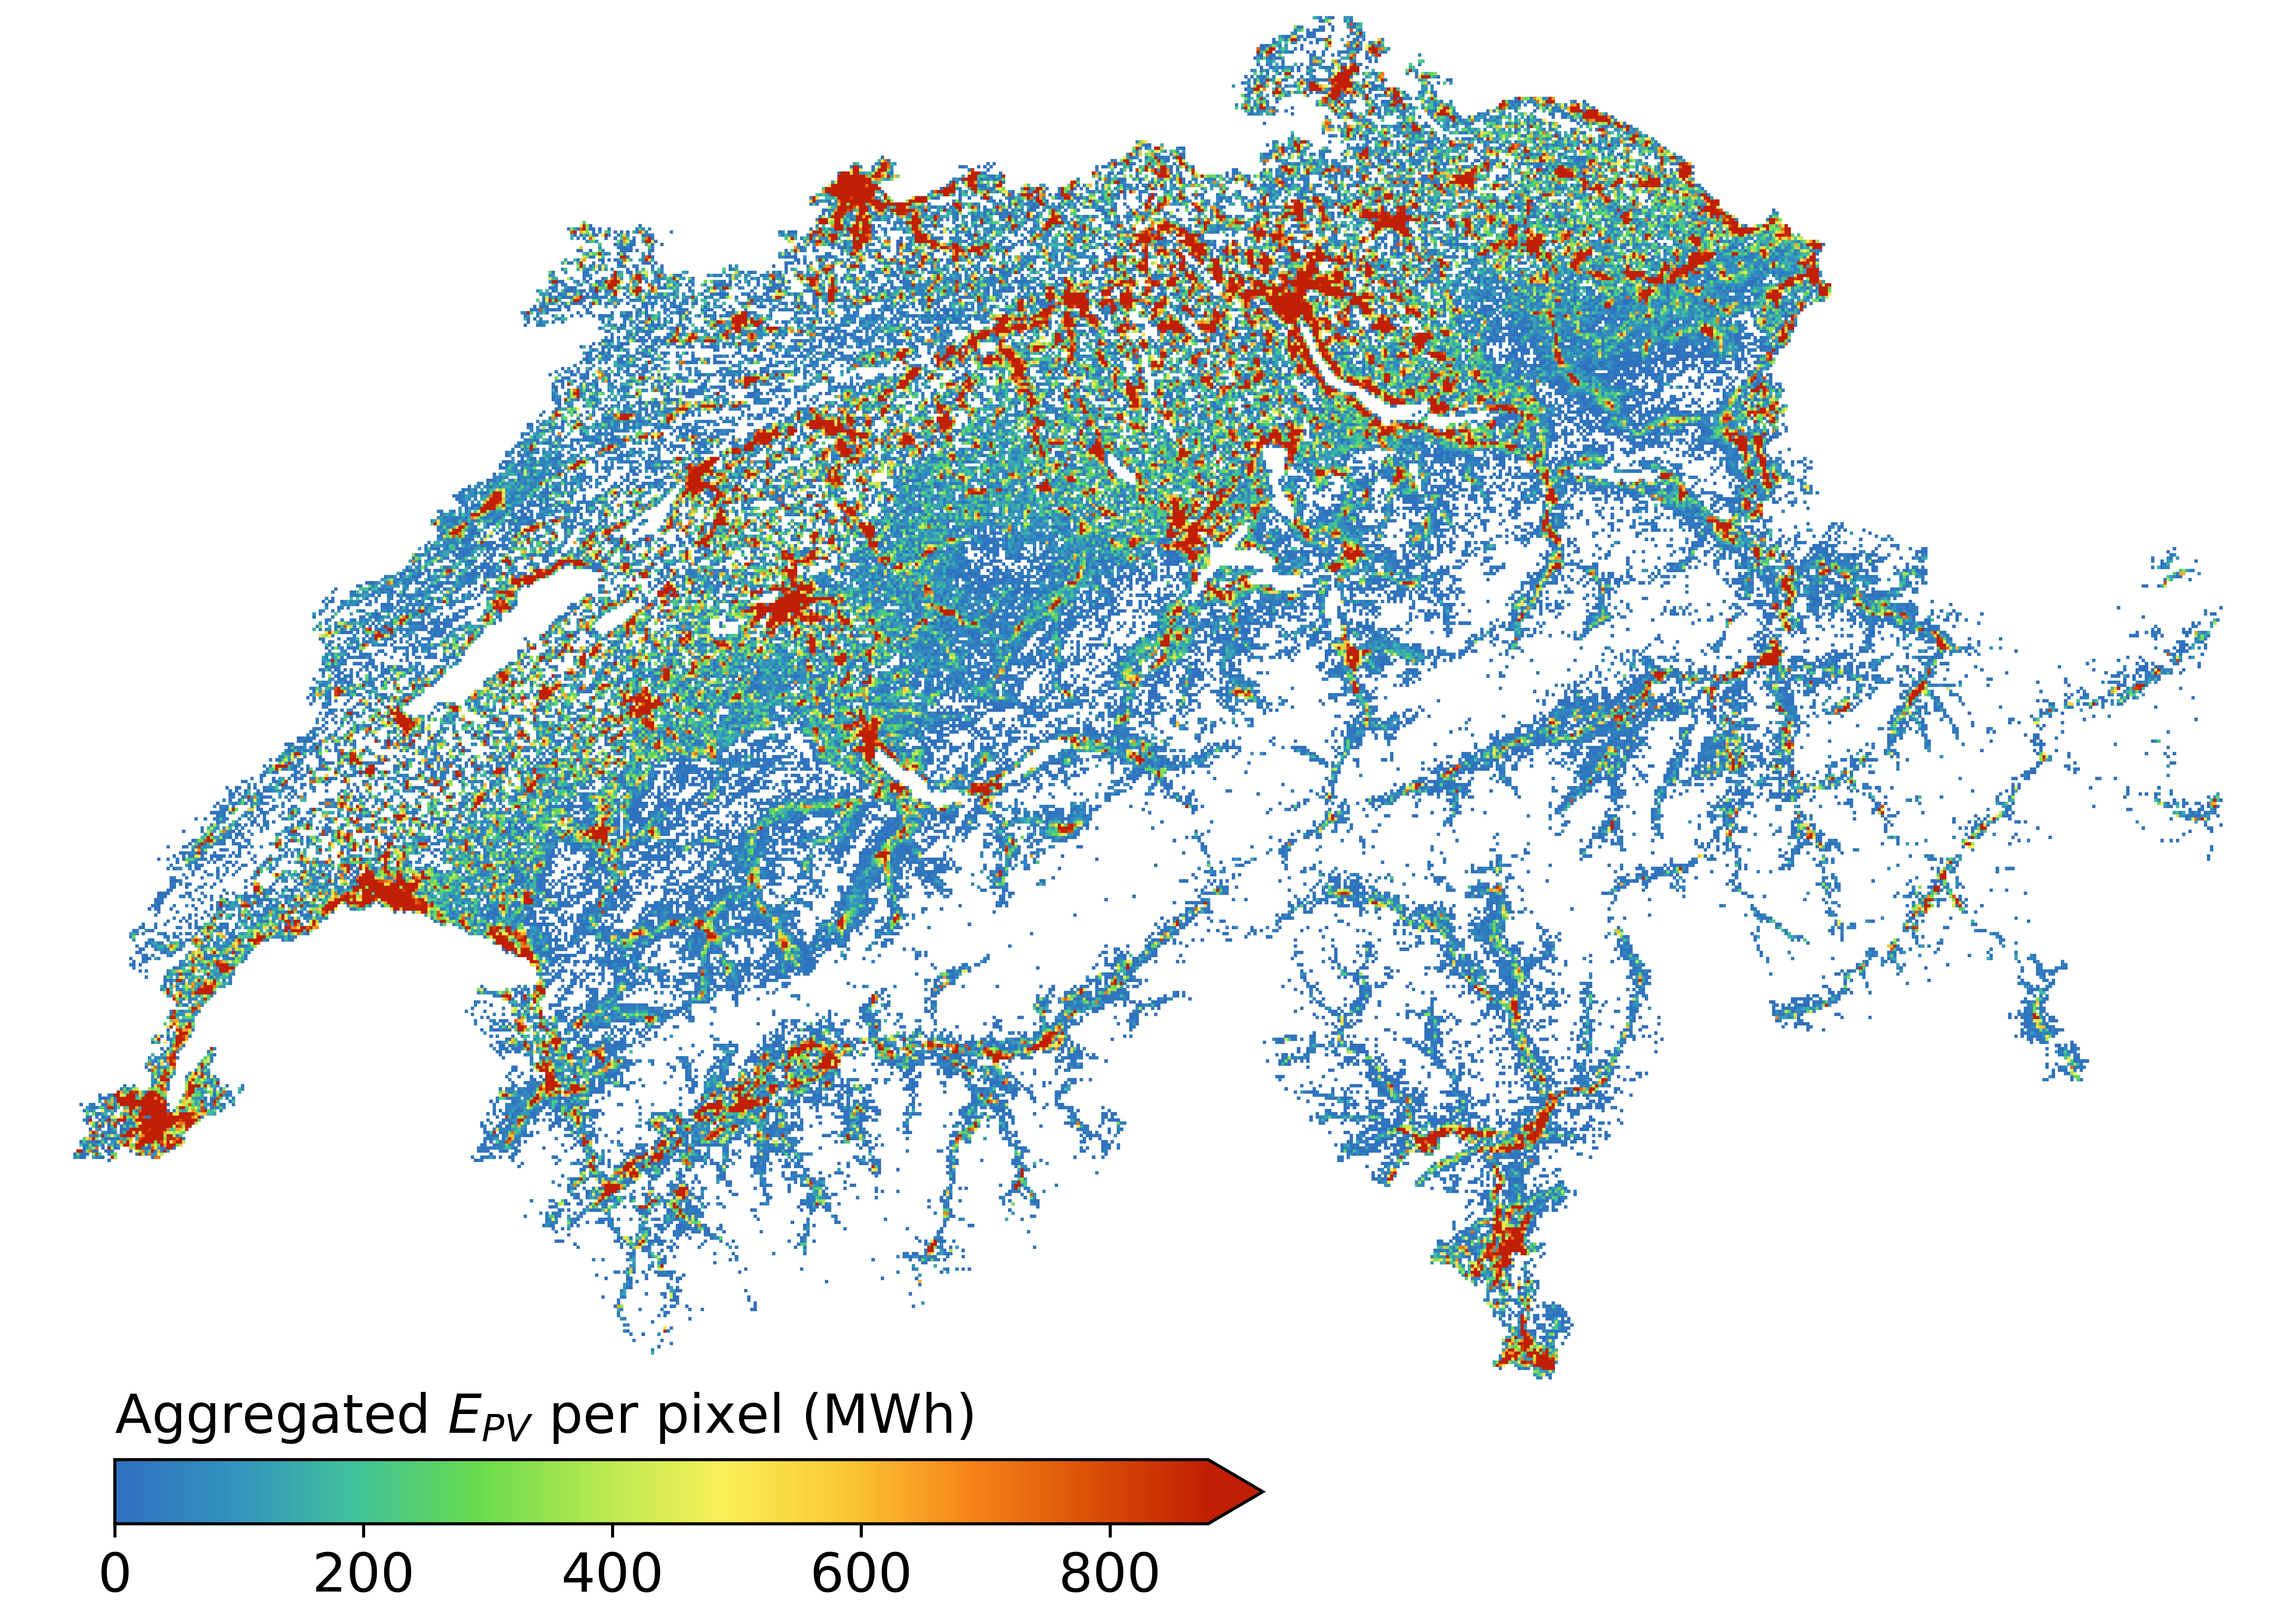
\includegraphics[width=0.98\linewidth]{Figs/PV_per_pixel_small.jpg}
  \subcaption{}
\end{subfigure}
\begin{subfigure}{.34\textwidth}
  \centering
  % include second image
  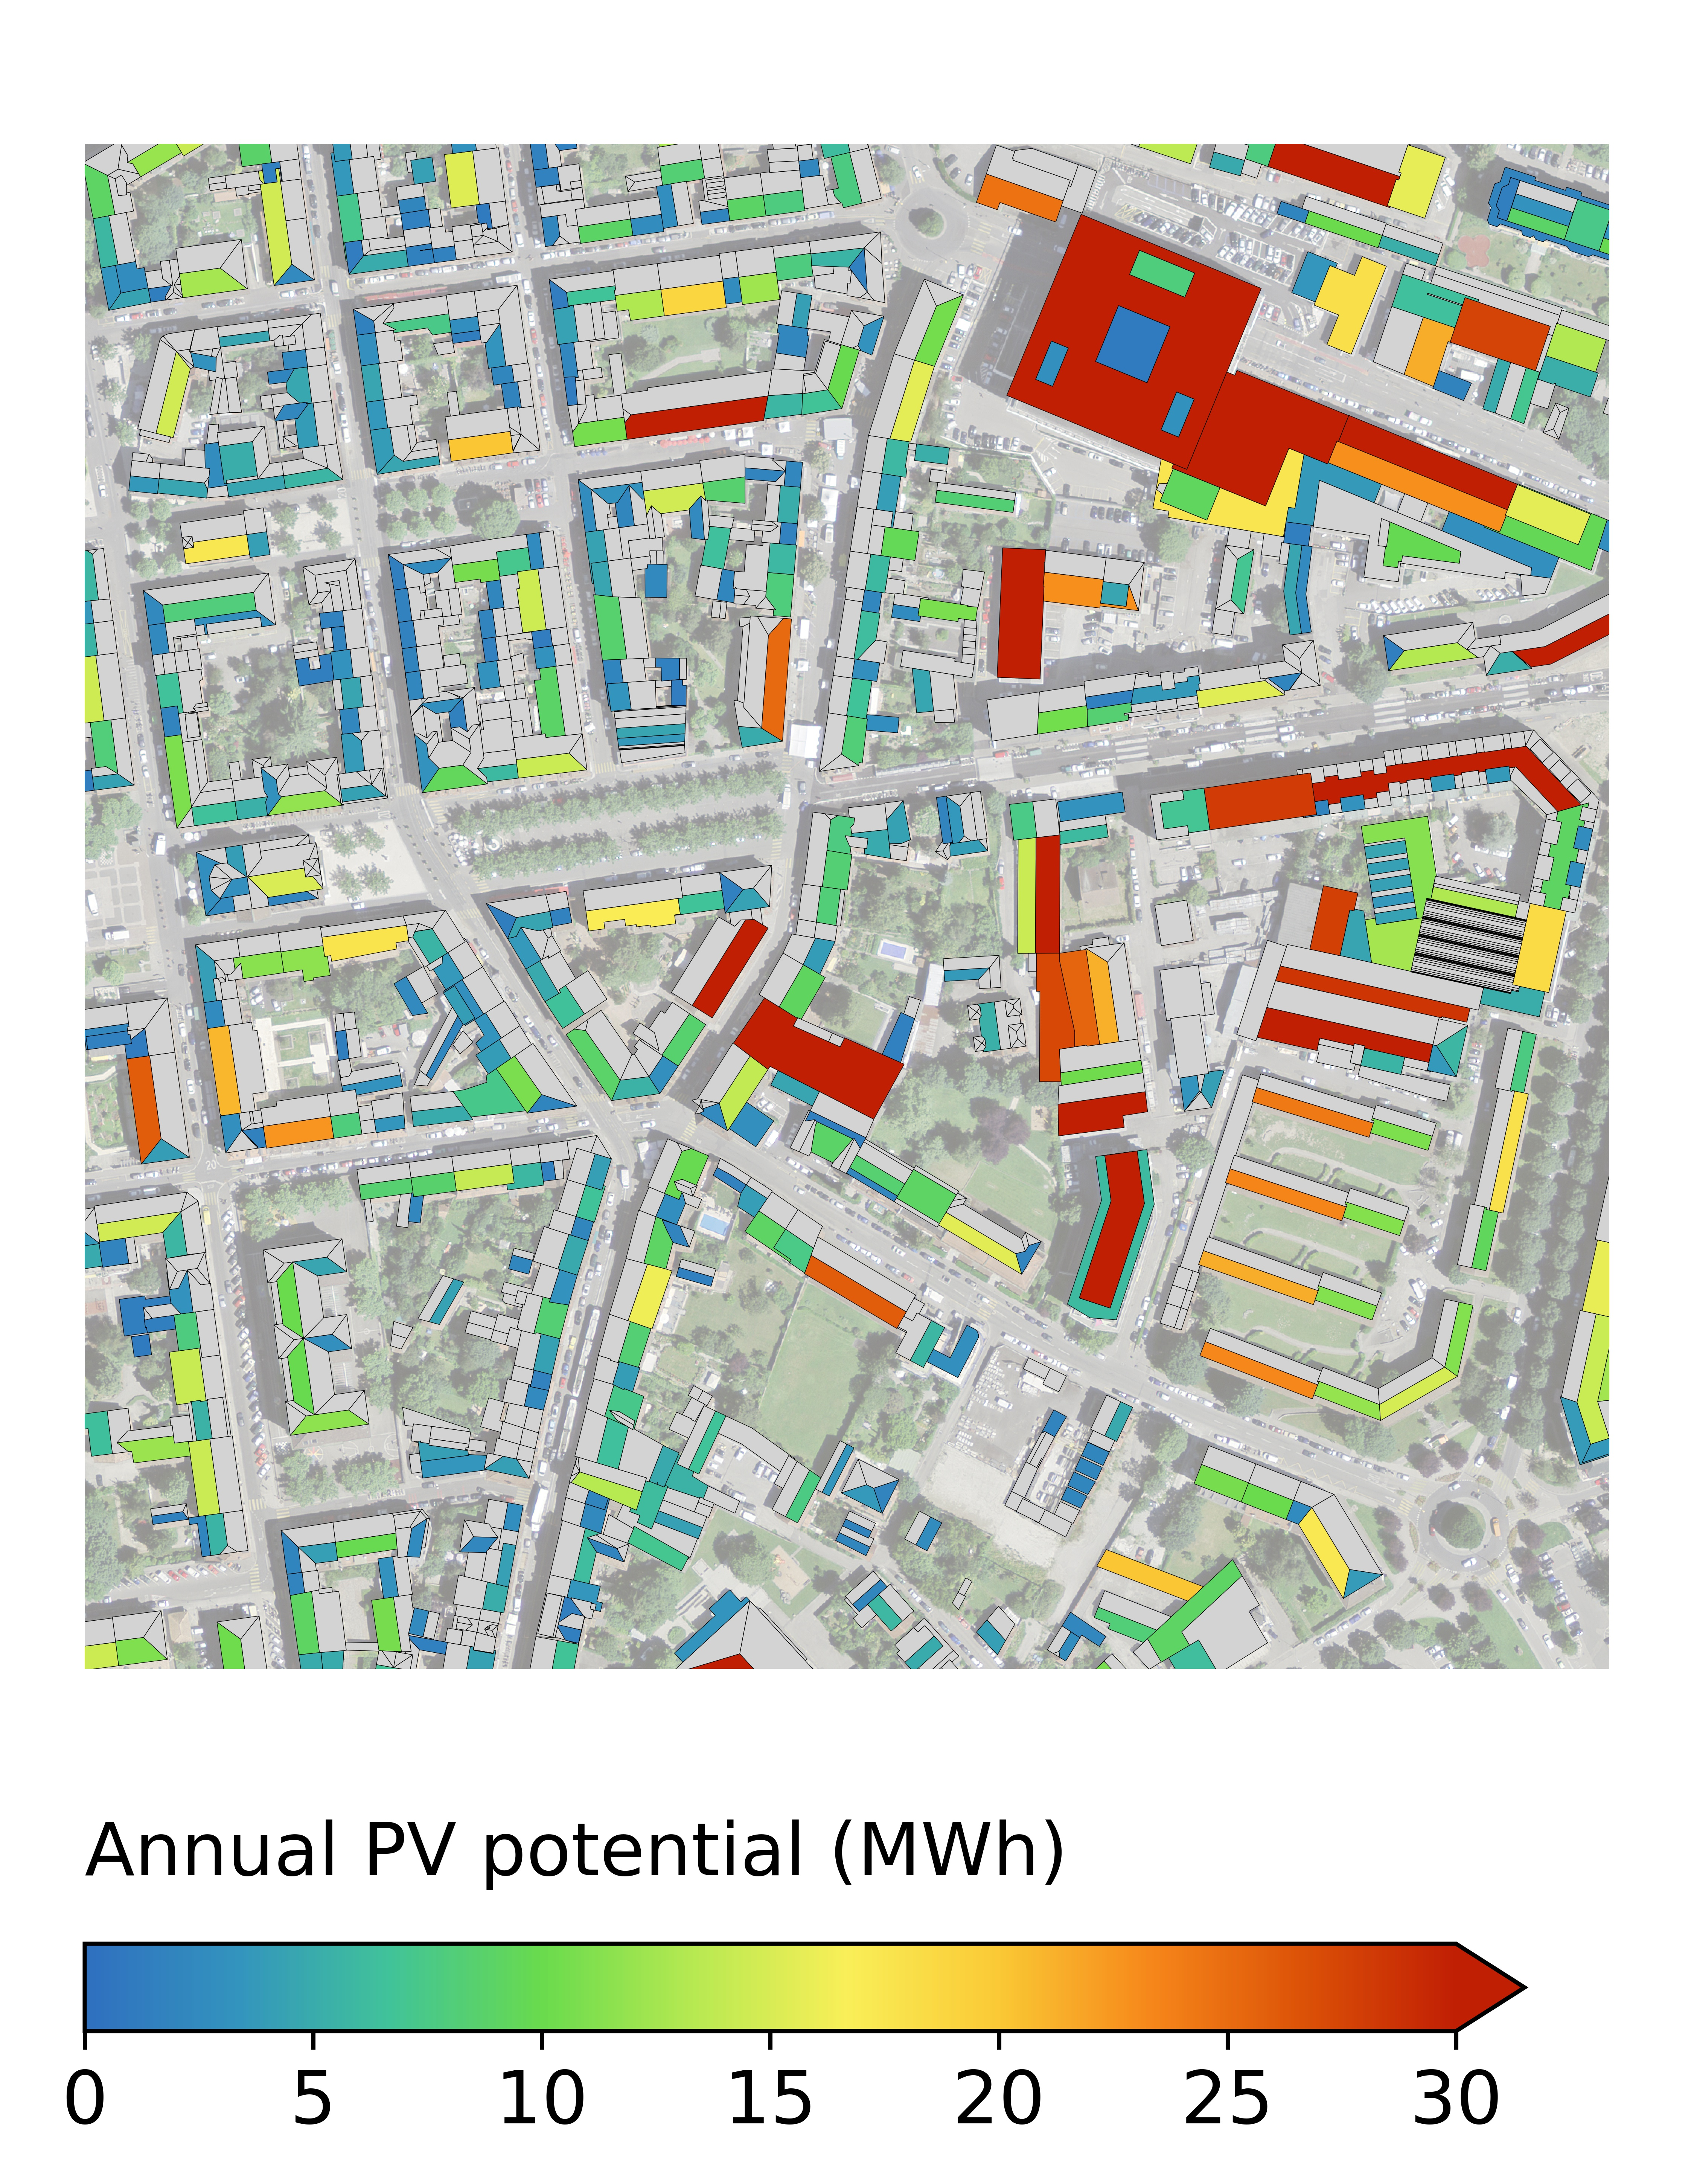
\includegraphics[width=0.98\linewidth]{Figs/PV_MWh_roofs.jpg}
  \subcaption{}
\end{subfigure}
\begin{subfigure}{.95\textwidth}
  \centering
  % include first image
  \includegraphics[width=\linewidth]{Figs/PV_hourly_w_unc_demand.pdf} 
  \subcaption{}
\end{subfigure}
\caption{a) Spatial distribution of annual $E_{PV}$, aggregated to pixels of $500 \times 500$ m$^2$ for visualization purposes, 
b) annual $E_{PV}$ for the suitable roofs of a randomly selected $500 \times 500$ m$^2$ pixel in the city of Geneva,
c) monthly-mean-hourly profiles of $E_{PV}$, summed for all suitable roofs, the $\sigma_{PV}$ and the Swiss electricity demand of 2018.}
\label{fig:results}
\end{figure}

\subsection{Sensitivity analysis}

We conduct a sensitivity analysis to quantify the impact of the individual parameters computed in this study on the technical PV potential. The analysis is performed in two stages: firstly, each parameter is independently varied in a fixed range of $\pm 50\%$. 
In a second step, all parameters with a quantifiable uncertainty are varied by $\pm \sigma$. 
Due to the high correlation of the horizontal radiation components, $G_h$ and $G_B$ are varied simultaneously. A representative sample of 10,000 rooftops has been used for this analysis.

Figure \ref{fig:sens_vars}a shows the change in technical PV potential for varying each parameter by $\pm 50\%$. The horizontal radiation components ($G_h$), and the fractions of available roof area ($C_{sh}, C_{\mathit{pv}}$) are the most sensitive parameters and thus exhibit the steepest slope. 
This is expected, as these variables are directly correlated with the factors in the computation of $E_{PV}$ (see Eq.~(\ref{eq:pv})). 
As the panel efficiency reduces slightly for high $G_h$, its sensitivity curve lies just below $C_{sh}, C_{\mathit{pv}}$.
Changes in $S_{sh}$ and $\mathit{SVF}$ have a smaller impact on the RPV potential, as they are multiplied with $G_{Bt}$ and $G_{Dt}$, respectively. 
The curves flatten out for large positive changes, as both factors are saturating at a value of 1. 
The albedo ($\rho$) has a very low sensitivity, as there are few steep roofs that are impacted by a change in $\rho$.
The ambient temperature ($T_{amb}$) is the only curve with a negative slope, as high temperatures decrease $\eta_{PV}$. Its sensitivity is rather low, as $T_{amb}$ only indirectly impacts the PV potential as part of the physical model of $\eta_{PV}$. 

\begin{figure}[tb]
\centering
\begin{subfigure}{.49\textwidth}
  \centering
  % include second image
  \includegraphics[width=\linewidth]{Figs/sensitivity_vars_Tamb.pdf}
  \subcaption{}
\end{subfigure}
\begin{subfigure}{.49\textwidth}
  \centering
  % include first image
  \includegraphics[width=\linewidth]{Figs/sensitivity_unc.pdf}  
  \subcaption{}
\end{subfigure}
\caption{Change in RPV potential for the variation of a) each variable by $\pm 50\%$ and b) each uncertain variable by $\pm \sigma$. Considered variables are the horizontal radiation ($G_h$), partly shading factor ($S_{sh}$), sky view factor ($\mathit{SVF}$), surface albedo ($\rho$), shaded and panelled area ratios ($C_{sh}, C_{\mathit{pv}}$) and ambient temperature ($T_{amb}$).}
\label{fig:sens_vars}
\end{figure}

Figure \ref{fig:sens_vars}b shows the impact of varying each variable within their uncertainty ($\pm \sigma$). 
The upper and lower dashed lines represent the propagated $\sigma_{PV}$. 
The results suggests that in a year with low $G_h$, the electricity generation may be up to 18\% lower than estimated, and similarly for the higher case. 
The $S_{sh}$ and $\mathit{SVF}$ show the lowest sensitivity, which agrees with Fig.~\ref{fig:sens_vars}a.
Comparing $C_{\mathit{pv}}$ and $C_{sh}$ shows that $\sigma_{\mathit{Cpv}}$, driven by the high uncertainty of medium-sized roofs, is overall larger than $\sigma_{\mathit{Csh}}$, with a potential impact of $\pm 11 \%$. 
%
The bars in Fig.~\ref{fig:sens_vars}b indicate the potential change when all roofs are considered, while the lines show the potential change for the suitable roofs only (see Section~\ref{tech}). 
For $G_t$, the suitable south-facing roofs have a higher uncertainty than all roofs, as expected from Fig~\ref{fig:Gt}b. 
The opposite is the case for $A_{PV}$, as the suitable roofs have a higher proportion of flat roofs with a low $\sigma_{\mathit{Cpv}}$.

%%%%%%%%%%%%%%%%%%%%%%%%%%%%%%%%%%%%%%%%%%%%%%%%%%%%%%%
%%%%%%%%%%%%%%%%%%%%%%%%%%%%%%%%%%%%%%%%%%%%%%%%%%%%%%%

\section{Discussion}
\label{discussion_pv}

\subsection{Methodological contribution}

Our methodology presents an end-to-end approach to estimate RPV potential at monthly-mean-hourly temporal resolution for individual roof surfaces. It uses large building and environmental datasets and may be transferred to any region or country where such data is or will become available. 
The proposed method adapts best existing practices for a data-driven estimation of each parameter that impacts RPV potential. This includes
(i) the spatio-temporal variation of the horizontal solar radiation,
(ii) the effects of surrounding trees and buildings on roof shading and the sky view factor,
(iii) the impact of roof geometry and superstructures on the available area for installing PV panels, and
(iv) the temperature-dependence of the PV module efficiency.
As a result, the potential computed here is more accurate and provides a higher spatio-temporal resolution than previous works.

The strength of our method lies in the combination of physical models with GIS and ML. The former two provide a detailed representation of the physical processes underlying the RPV assessment. The use of ML, applied previously only in \cite{assouline_quantifying_2017, assouline_large-scale_2018}, allows to include additional knowledge extracted from data with only partial spatial or temporal coverage, and hence improves the accuracy of the results. 
The ML approach also outlines a method to use sparsely available datasets for a PV assessment in other regions.

Furthermore, we propose a structured method to estimate and propagate uncertainty in large-scale PV potential studies. Using the ML and GIS methods, we are able to quantify uncertainties related to the data sources and individual processing steps. These values are then combined using statistical tools to estimate the total uncertainty.
This allows decision-makers to better understand the potential contribution of RPV to future energy systems. 

%%%%%%%%%%%%%%%%%%%%%%%%%%%%%%%%%%%%%%%%%%%%%%%%%

\subsection{Practical contribution}

The application of the methodology to Switzerland provides several practical contributions for an effective integration of RPV in the built environment. 
Firstly, our results form a dataset of hourly profiles of RPV potential and its uncertainty for 9.6M rooftops in Switzerland, which will be publicly accessible. To the best of our knowledge, it is the first dataset of its type at this spatio-temporal resolution and scale. Our data can be used by the research community to study future energy systems with large shares of RPV, whereby the uncertainty permits the modelling of different scenarios. 

Secondly, the large-scale estimate of $24 \pm 9$ TWh provides a realistic estimate of the maximum technical RPV potential for Switzerland. According to our data, electricity generation from PV may cover over 40\% of Switzerland's annual demand of 57.6TWh in 2018 \cite{swiss_federal_institue_for_energy_schweizerische_2018}. However, our results also show that the potential contribution from RPV is insufficient during winter and night hours, while there may be a large surplus of RPV generation during peak hours in summer (see Fig~\ref{fig:results}b).

Thirdly, the sensitivity analysis performed here identifies the parameters with the highest impact on the estimated RPV potential, as well as the main sources of uncertainty (see Fig.~\ref{fig:sens_vars}). The parameter with the highest impact is the horizontal radiation. Its uncertainty is mainly caused by the high intermittency of the solar resource and can not be significantly reduced, even if higher-quality data was available. 
The panelled area ratio represents the second largest source of uncertainty. In this case, it is due to inaccuracies in the input data and uncertainty in the modelling approach. These may be reduced by a more precise model, for example using image processing techniques \cite{mainzer_assessment_2017}, or a more detailed building model (i.e. LOD 4) that is available in the entire study region.

\begin{comment}
% MOVED TO SEPARATE SUB-SECTION
\subsection{Comparison with existing studies}
\label{comparison}

\begin{table}[b]
\centering
\footnotesize
\caption{Comparison of the results presented in 6 studies of technical RPV potential in Switzerland. To obtain comparable results, the entries labelled with * are computed from values quoted in the respective publications as explained in \cite{walch_critical_2019}.}
\label{tab:comparison}
\begin{tabular}{lccccc}
\hline
 & \textbf{$\mathbf{A_{PV}}$} & \textbf{Suitable} & \textbf{$\mathbf{G_t}$} & \textbf{$\boldsymbol{\eta_{sys}}$} & \textbf{$\mathbf{E_{PV}}$} \\
\textbf{Study}           & (km$^2$) & \textbf{roofs} (\%) & (kWh/m$^2$) & (\%) & (TWh) \\
\hline
\citet{iea_potential_2002}             & 251*               & 55                   & 1,088*             & 10                   & 15.04                   \\
\citet{assouline_quantifying_2017}             & 328                & 60.5*                & 662*               & 13.6                 & 17.86                   \\
\citet{assouline_large-scale_2018}             & 252                & 60.5*                & 786*               & 13.6                 & 16.29                   \\
Sonnendach \cite{klauser_solarpotentialanalyse_2016, portmann_sonnendach.ch:_2016}    & 439*               & 71.6*                & 1,243*             & 13.6                 & 53.09*                  \\
\citet{buffat_scalable_2018}            & 485                & 70.1*                & 1,176*             & 10.3                 & 41.20*                  \\
Present study        & 267                & 56.4                 & 1,186              & 13.8                 & 24.58                   \\ \hline
\end{tabular}
\end{table}

To set our large-scale estimate into context, we compare it to five national studies on RPV potential in Switzerland \cite{iea_potential_2002, assouline_quantifying_2017, assouline_large-scale_2018, klauser_solarpotentialanalyse_2016, buffat_scalable_2018}, including a national project known as \textit{Sonnendach/toitsolaire}~\cite{klauser_solarpotentialanalyse_2016, portmann_sonnendach.ch:_2016}. This allows to validate the magnitude of our results against existing work and to point out the improvements achieved through our methodology.
Table~\ref{tab:comparison} shows a quantitative comparison of all studies, which is further detailed in \cite{walch_critical_2019}. The metrics used for comparison are the total available area ($A_{PV}$), the percentage of total roof surface that is suitable for installing PV, the annual tilted irradiation ($G_t$), the system efficiency ($\eta_{sys}$), which combines module efficiency and performance factor, and the annual PV potential ($E_{PV}$). 

Our results lie in the mid-range of the existing work. Using high-resolution building data shows that $A_{PV}$ is relatively low in comparison with other studies. It is in the range of the estimates by Assouline et al. \cite{assouline_large-scale_2018, assouline_quantifying_2017}, which use similar data-driven methods for estimating $A_{PV}$ as applied here. This suggests that the ratio of available roof area for PV installation lies much below current expert recommendations, which are used in \cite{portmann_sonnendach.ch:_2016}. This may be due to the fact that current recommendations are focused on roofs with a high potential, which may not be representative for all roofs in the Swiss building stock. In \cite{buffat_scalable_2018}, the available area for PV is not specifically addressed.

The annual tilted irradiation is relatively high and comparable to that estimated by \citet{klauser_solarpotentialanalyse_2016} and \citet{buffat_scalable_2018}. Both studies apply best practices for the estimation of shading effects and use high-resolution satellite data. A validation of $G_t$ against measurement data is provided in \cite{buffat_scalable_2018}, who find a negligible mean error in summer when production is highest, and a small overestimation in winter. 
This suggests that the annual irradiation is close to its real value, while it is likely underestimated in \cite{iea_potential_2002, assouline_quantifying_2017, assouline_large-scale_2018}, possibly due to a different computation of the shading effects.

Several complementarities exist between this study and previous work, given by the use of similar datasets and methods. This leads to comparable aggregated values and allows for the validation of our results against existing approaches.
The added value of our work is given firstly by the computation of the results in monthly-mean-hourly resolution, instead of yielding monthly or yearly values as used in \cite{klauser_solarpotentialanalyse_2016, assouline_quantifying_2017, assouline_large-scale_2018}. Secondly, we contribute to the existing work by assessing the available area for PV installation for each roof surface, rather than using communes~\cite{assouline_quantifying_2017} or pixel sizes of $200 \times 200$ m$^2$~\cite{assouline_large-scale_2018}. Thirdly, our study is the only one that quantifies the uncertainty on the final potential estimate. 
Uncertainties are not specifically addressed in \cite{assouline_quantifying_2017, assouline_large-scale_2018, iea_potential_2002} and qualitatively assessed in \cite{klauser_solarpotentialanalyse_2016, buffat_scalable_2018}.
\end{comment}

%%%%%%%%%%%%%%%%%%%%%%%%%%%%%%%%%%%%%%%%%%%%%%%%%%%%%%%

\subsection{Limitations}
\label{limitations_pv}
As all large-scale potential studies, our study relies on various data sources and a combination of statistical and empirical modelling steps. In this work, emphasis has been placed on systematically identifying and combining uncertainties in order to obtain a global uncertainty estimate for the technical RPV potential. 
Furthermore, a sensitivity analysis has been conducted to assess the impact of the uncertainty of individual steps on the final potential. 

Some assumptions were made that impact these results:
(i) The input data is assumed to be coherent and without error. In reality, some features may be missing or incorrectly represented, and discrepancies between the datasets may arise from  different data collection dates and methods of creation.
(ii) The systematic error introduced by using a fixed number of azimuth angles for computing the shading effects (38 bins) and the SVF (32 bins) is neglected. This error is expected to be negligible as the number of bins used here is relatively high.
(iii) The potential uncertainties arising from the physical models of tilted radiation and module efficiency are neglected, as no comprehensive quantification of these has been found in the literature.
(iv) The PV panel performance parameters as well as the system losses are treated as assumptions rather than random variables, due to the large variety of available technologies and their fast development. 
(v) PV panels on flat roofs are all placed in a technically optimal fashion (see Section~\ref{flat}). 
A comparison with other installation practices, such as lower tilt angles or the alternation of east and west-facing rows, is beyond the scope of this work.
To consider different configurations of PV on flat roofs and the uncertainty in technological developments, a scenario-based approach may be followed (see Section\ref{solar_scenarios}).

%%%%%%%%%%%%%%%%%%%%%%%%%%%%%%%%%%%%%%%%%%%%%%%%%%%%%%%

\subsection{Application and further work}
\label{application_pv}
% REFER TO FURTHER WORK DONE IN THE NEXT SUB-SECTION
A monthly-mean-hourly technical RPV potential for Switzerland is useful for applications including policy making, urban planning and the design of future energy systems. 
Policy makers may use our results, aggregated at regional or national scale, in order to formulate effective policies to integrate RPV into the built environment. 
Urban planners may assess the potential self-consumption and the electricity demand which could be covered by installing PV on existing roofs. They may further estimate the expected PV yield for new roofs of a given area, tilt and orientation from our results. 
Energy system designers can use this work to simulate future electricity networks at local scale, which allows to assess the potential mismatch between supply and demand and the resulting storage needs. 

The generated dataset may be further used to estimate the PV potential for future scenarios that account for urbanization, climate change and technological advancement of PV.
This is possible as the existing building stock covers different types of roofs in various urban contexts and climatic conditions, which exist in the Swiss plateau, the Jura mountains and the Alps. 
A techno-economic potential may be formulated for these scenarios by combining the maximum technical potential with economic factors such as installation and operational cost.

Finally, a further validation of the estimated RPV potential provides a challenging subject of future work. 
We validate our results against those of previous work (Section~\ref{comparison}), some of which have been compared to measurement data \cite{buffat_scalable_2018}. While this approach is feasible for validating the tilted radiation, a direct validation of the available area is difficult due to the lack of a "ground truth". A possible method to establish such a ground truth may be the application of image segmentation techniques, for example using Convolutional Neural Networks \cite{castello_deep_2019}, to high-resolution aerial imagery. 
This would allow for a more accurate detection of obstructing objects on rooftops as well as the recognition of already installed PV panels (see Section\ref{solar_scenarios}).

%%%%%%%%%%%%%%%%%%%%%%%%%%%%%%%%%%%%%%%%%%%%%%%%%%%%%%%
%%%%%%%%%%%%%%%%%%%%%%%%%%%%%%%%%%%%%%%%%%%%%%%%%%%%%%%


\section{Comparison to existing studies}
\label{solar_comparison}

\begin{comment}
Installing photovoltaics (PV) on building rooftops is a promising approach to reduce greenhouse gas emissions, especially in dense urban areas. Understanding the large-scale potential for rooftop PV is important for several reasons, including electricity network design, urban and regional energy planning, as well as incentive policies for PV installations. Several studies in recent years focus on assessing a large-scale technical rooftop PV potential. Early methods relying on “rules of thumb” \cite{iea_potential_2002} have been continuously improved by incorporating environmental and building data as well as using powerful computational engines and advanced analytic methods such as Machine Learning (ML). This progress in data processing, enabled by the availability of larger and more accurate datasets, has led to widely varying results of PV potential studies, even for the same geographic area. This makes the comparison across studies intrinsically challenging. \citet{assouline_estimation_2017} provide an overview of the existing methods to estimate a large-scale technical rooftop PV potential, however this methodological review does not discuss the results obtained by individual studies. Some of these compare their results with those of other studies, but the discrepancies are explained in a qualitative rather than quantitative way \cite{assouline_quantifying_2017,assouline_large-scale_2018}. 
\end{comment}

In this paper, we propose a framework to compare large-scale rooftop PV assessment studies in a quantitative way. This helps us to understand how different methods impact the potential estimates. We focus our comparison on Switzerland, where six different studies have been carried out at national scale from 2002 to 2019 \cite{iea_potential_2002,assouline_quantifying_2017,assouline_large-scale_2018,klauser_solarpotentialanalyse_2016,buffat_scalable_2018, walch_big_2020}. The results are interpreted with respect to the following aspects: (i) target audience, (ii) spatio-temporal resolution, (iii) datasets, and (iv) methods. We finally provide a perspective on future developments which may further improve the PV potential studies. In Switzerland, the following six studies have been conducted at different scales. 

\begin{enumerate}
\item The first study (\textit{\textbf{S1}}) was conducted for several European countries including Switzerland by the International Energy Agency (IEA) in 2002 \cite{iea_potential_2002}. The method is based on rules of thumb, established at European scale, and does not reflect the local building stock characteristics within Switzerland. The technical potential is given as a yearly value for the entire country, representing the lowest temporal and spatial resolution among the compared studies. It is aimed at indicating an order of magnitude of the total technical rooftop PV potential at national scale. 
\item The second study (\textit{\textbf{S2}}) for Switzerland was conducted by \citet{assouline_quantifying_2017} at commune scale. In this study, a Machine Learning algorithm, Support Vector Machines (SVM), combined with Geographic Information Systems (GIS), is used in order to estimate the technical PV potential on building rooftops. ML is used as an effective method of extrapolation to solve problems of data availability in parts of the study area. The study is performed at monthly-mean-daily temporal resolution for all Swiss communes. 
\item The third study (\textit{\textbf{S3}}) is again conducted by \citet{assouline_large-scale_2018} at $200 \times 200$ m$^2$ spatial resolution. In this study, another ML algorithm, Random Forests (RF), is used in combination with GIS to estimate the potential. The method from S3 is enhanced in S4 using (i) larger and more accurate datasets, (ii) a more efficient  ML algorithm that includes the estimation of model uncertainties, and (iii) a higher spatial resolution of $200 \times 200$ m$^2$. Both studies aim at a large-scale estimation of PV potential on building roofs to inform regional and national decision making.
\item The fourth study (\textbf{\textit{S4}}) was conducted as a national project, namely Sonnendach.ch, by the Swiss Federal Offices of Energy (SFOE), Topography (Swisstopo), and Meteorology and Climatology (MeteoSwiss) \cite{klauser_solarpotentialanalyse_2016,portmann_sonnendach.ch:_2016}. Monthly solar PV potential is estimated for each rooftop in Switzerland using a GIS-based approach \cite{klauser_solarpotentialanalyse_2016} complemented by rules of thumb \cite{portmann_sonnendach.ch:_2016}. In contrast to the above studies (S1-S3), the primary target group of this study is individual property owners and energy service providers interested in installing PV on specific building roofs. Thus, the primary output of this study is a classification of rooftop suitability for solar PV installation.
\item The fifth study (\textbf{\textit{S5}}), conducted by \citet{buffat_scalable_2018}, estimates PV potential from solar radiation profiles in half-hour temporal resolution for pixels of $0.5 \times 0.5$ m$^2$. In this study, GIS is used to estimate the solar radiation on tilted surfaces. In addition, the study includes a detailed model of the panel and inverter efficiencies. The results presented in the study aim primarily at a comparison between different PV technologies and are validated against measurement data.
\item The sixth study (\textbf{\textit{S6}}) has been carried out by \citet{walch_big_2020} based on a big data approach. In this study, Geographic Information Systems and Machine Learning approaches are used to estimate the solar PV potential for each building roof surface at hourly temporal resolution. ML is used to quantify not only the modelling uncertainty for the resulting PV potential estimation, but also the uncertainty in the data. The hourly temporal resolution of the results is very important for the spatio-temporal modelling of future electricity systems.   
\end{enumerate}

\subsection{Methodological comparison}

To compute the technical rooftop PV potential, a hierarchical approach has been widely accepted in the literature and is used in all studies. It includes (i) physical potential, that is, the amount of solar energy reaching the earth’s surface, (ii) geographic potential, that is, the amount of solar radiation received by the tilted PV panels, which is affected by the geometry of the panel (slope and aspect), the shading from surrounding buildings and trees and the suitable area for the panel installation, and (iii) technical potential, that is, the maximum electricity output considering the technical characteristics of the PV technology (e.g. efficiency and system performance).

The physical potential is defined as the global horizontal solar radiation ($G_h$), consisting of a direct horizontal ($G_B$) and a diffuse horizontal ($G_B$) component. In S1, a constant $G_h$ of 1,167 kWh/m$^2$ (from Meteonorm) is used for the entire country. In all other studies (S2-S6), the three horizontal radiation components $G_h$, $G_B$ and $G_B$ are obtained from satellite-derived solar radiation data based on the Heliosat algorithm \cite{rigollier_method_2004}. S2 and S3 use the mentioned data for 100 locations, S5 uses a gridded dataset at $3.8 \times 5.6$ km$^2$ spatial resolution (SARAH) and S4 and S6 use satellite data on a $1.6 \times 2.3$ km$^2$ grid provided by MeteoSwiss, which contains improvements for radiation modelling at high altitude \cite{stockli_heliomont_2017}. S4 and S5 directly use the input data as physical potential. S2, S3 and S6 use Machine Learning to derive $G_h$, $G_B$ and $G_B$ on a $200 \times 200$ m$^2$ grid to better represent the local terrain. In S2 and S3, additional measurements of temperature, precipitation, sunshine duration and cloud cover are used to support the estimation, while S6 use exclusively spatial features, namely longitude, latitude and altitude. 

The geographic potential is driven by two factors: (i) tilted radiation, that is, the solar radiation on a tilted PV panel ($G_t$, in kWh/m$^2$) and (ii) available area for PV panel installation ($A_{PV}$, in m$^2$). $G_t$ and $A_{PV}$ for a rooftop PV potential estimation may be generally defined as:

\begin{equation}
\label{eq:Gt_compare}
    G_t = (1 - Sh_A) (Sh_{Bt} * G_{Bt} + \mathit{SVF} * G_{Dt} + G_{Rt})
\end{equation}

\begin{equation}
\label{eq:APV_compare}
    A_{PV} = A_{\mathit{floor}} * C_R \quad \forall A_{PV} > A_{min} 
\end{equation}

where $G_{Bt}$, $G_{Dt}$ and $G_{Rt}$ are the direct, diffuse and reflected tilted radiation components, $Sh_A$ and $Sh_{Bt}$ are parameters of shading losses, explained below, \textit{SVF} denotes the sky view factor, $A_{\mathit{floor}}$ is the ground floor area, $C_R$ denotes the ratio of available area for PV panel installation over ground floor area and $A_{min}$ describes the minimum roof area considered for PV installation. Despite following the same physical principles, differences in spatio-temporal resolution and available datasets lead to significantly varying methods for calculating the parameters for geographic potential, as summarized in Table \ref{tab:compare_methods}. It should be noted that probabilistic functions are used in S2 and S3 to compute the geographic potential as detailed roof shapes are unknown. One exception to Eqs.~\ref{eq:Gt_compare} and \ref{eq:APV_compare} is S1, where the geographic potential is computed in a simplified way. In S1, $G_t$ is obtained by multiplying $G_h$ with an average solar yield ($\sim 93.3\%$ for Switzerland, derived from \cite{iea_potential_2002}). $A_{PV}$ is computed by multiplying an estimated floor area (45 m$^2$ per person) with the population size and a constant ratio of “architecturally suitable area / ground floor area”, equal to 0.72. This accounts for construction elements (here $C_R$) as well as shading (here $Sh_A$) \cite{iea_potential_2002}.

In S2-S6, shading effects ($Sh_A$, $Sh_{Bt}$) are computed separately from $C_R$ using GIS and a Digital Elevation Model (DEM).  All studies use Switzerland’s DEM in $2 \times 2$ m$^2$ resolution, which was created by Swisstopo. S4 and S5 interpolate this DEM to a $0.5 \times 0.5$ m$^2$ resolution. We distinguish between two types of shading, namely (i) the fraction of a roof area in full shade ($Sh_A$), and (ii) the average amount of shading on the remaining roof ($Sh_{Bt}$), reducing the direct tilted radiation. $Sh_A$ is only considered in S2, S3 and S6. S2 and S3 follow a Hillshade (HS) approach which estimates shading by computing relief maps for each pixel of a Digital Elevation Model (DEM). $Sh_A$ is obtained from pixels with a HS value of 0, while $Sh_{Bt}$ is obtained by averaging the remaining pixels over a building roof. ML is used by S2 and S3 to estimate shading effects at commune and pixel scale for Switzerland based on data from Geneva Canton. In contrast, S4-S6 use a horizon-based method, where binary maps of sun visibility are computed for each hour and each pixel of a DEM. S5 directly uses these binary maps to compute the per-pixel tilted radiation, so $Sh_{Bt} \in {0, 1}$. S4 and S6 average the results for each roof such that $Sh_{Bt} \in [0, 1]$. $Sh_A$ is computed in S6 as areas with low sunlight exposure, i.e. $\bar{Sh_{Bt}} < 40\%$. SVF, which reduces the diffuse tilted radiation, is accounted for in S2 and S3 through a constant (0.9) and in S4 and S6 by using GIS. $G_{Bt}$, $G_{Dt}$ and $G_{Rt}$ are computed in S2 and S3 from daily solar radiation models [3,4]. S4-S6 use hourly models, explained in \cite{perez_modeling_1990}, and apply the anisotropic Perez model for the diffuse component.

The available roof area for PV panel installation is estimated in each study to a different extent. S5 does not compute any $C_R$, while S4 uses roof-specific rules of thumb based on expert knowledge, which are in the range of 0.42-0.8 \cite{portmann_sonnendach.ch:_2016}. S2, S3 and S6 use a combination of GIS and ML to obtain $C_R$. GIS is used in S2 to remove superstructures (SP) from roof polygons and to compute the resulting useful roof area. S3 improves on S2 by virtually installing PV panels (VP) on the building roofs. In both cases, the GIS algorithms are applied to all rooftops in Geneva Canton, where detailed city GML data (LOD 4) is available. ML is then used to estimate $C_R$ in all other communes/pixels based on building characteristics, which are derived from the Swiss building registry (RegBL). In contrast, S6 uses roof data for the entire country to virtually install panels, reducing the uncertainty related to estimating $C_R$ with respect to S2 and S3. ML is applied in S6 to consider superstructures at national scale, by extrapolating the change in $C_R$ when accounting for SP, which is again computed for Geneva Canton where LOD 4 data is available.
The technical potential is computed as shown in Eq.~\ref{eq:EPV_compare} by multiplying $G_t$, $A_{PV}$, the module efficiency ($\eta$) and a performance factor (\textit{PF}), which accounts for losses of the inverter, soiling, degradation, etc. Most studies approximate $\eta$ and \textit{PF} using constants. S5 and S6 use physical models for module and inverter efficiencies. S5 further compares the results for monocrystalline, poly-crystalline and thin film technologies. From an economic point of view, it is necessary to exclude unsuitable surfaces when estimating the solar rooftop PV potential. In S1, unsuitable surfaces are defined as those with a yield below 80\%, which is approximated to be 55\% of roofs \cite{iea_potential_2002}. S2, S3 and S6 define suitable roofs as those facing southwards, with an aspect angle of $\pm 90^\circ$ (east to west), while S4 and S5 exclude those roofs/pixels with an annual tilted radiation below 1,000 kWh (see Table~\ref{tab:compare_methods} for reference).

\begin{table}[htb]
\centering
\footnotesize
\caption{Comparison of methods for computing the main parameters of rooftop PV potential.}
\label{tab:compare_methods}
\begin{tabular}{lcccccc}
\hline
\textit{\textbf{Parameter}} & \textbf{S1}           & \textbf{S2}                     & \textbf{S3}   & \textbf{S4}          & \textbf{S5}    & \textbf{S6}         \\ \hline
$G_{Bt}, G_{Dt}, G_{Rt}$               & $G_h$ * \textit{yield}            & Daily                           & Daily         & Hourly               & Hourly         & Hourly              \\
\textit{SVF}                & -                     & 0.9                             & 0.9           & Horizon              & 1              & 0.9                 \\
$Sh_{Bt}$                        & -                     & Hillshade                       & Hillshade     & Horizon              & Horizon        & Horizon             \\
$Sh_A$                         & \multirow{2}{*}{0.72} & Hillshade = 0                   & Hillshade = 0 & 0                    & 0              & $\overline{Sh}_{Bt}$ \textless   40\% \\
$C_R$                          &                       & SP                              & SP + VP       & 0.42 – 0.8           & 1              & SP + VP             \\
$A_{min}$                        & -                     & 28 m$^2$                            & 8 m$^2$           & 10 m$^2$                 & -              & 8 m$^2$                 \\
\textit{Suitable roofs}     & 55\% of roofs         & roof aspect $\in [-90^\circ,   90^\circ]$ &               & $G_t$ \textgreater 1000 &                & as S2/S3            \\
$\eta$                      & \multirow{2}{*}{10\%} & 17\%                            & 17\%          & 17\%                 & Panel model    & Panel model         \\
\textit{PF}                 &                       & 80\%                            & 80\%          & 80\%                 & Inverter model & Inverter model      \\ \hline
\end{tabular}
\end{table}

\begin{equation}
\label{eq:EPV_compare}
    E_{PV} = G_t * A_{PV} * \eta * \mathit{PF} \quad \forall suitable roofs
\end{equation}

Finally, the number of buildings considered in each study and the type of dataset used to describe buildings/roofs is important, as it impacts the total floor area ($A_{\mathit{floor}}$) and hence the order of magnitude of final PV potential. Again, S1 applies a rule of thumb of $A_{\mathit{floor}} = 45$ m$^2$ per capita. S2 uses polygons of building clusters (Vector25) in urban areas only. S3 uses a combination of these building clusters and roof surface polygons with a higher spatial resolution, representing a total of nearly 2 million buildings in Switzerland \cite{assouline_large-scale_2018}. The estimation in S5 is based on individual building footprints for the entire country, mostly from the Swiss cadastral survey. S4 and S6 use a national dataset of 9.6M roof surface polygons, representing 3.7M buildings, which was derived from a national 3D building model (LOD 2) by Swisstopo . It should be noted that the building footprint area in S5 is lower than the total building area declared by the Swiss Federal Statistical Office (2009 estimate) \cite{buffat_scalable_2018}. In contrast, the national roof surface dataset used in S3 (partly), S4 and S6 may overestimate total roof area, as some polygons overlap \cite{swisstopo_swisstlm3d_2018}.

\subsection{Quantitative comparison}

\subsubsection{Metrics of comparison}

The quantitative comparison of the studies, shown in Table~\ref{tab:compare_values}, is performed in terms of the main factors defined in Eqs.~\ref{eq:Gt_compare}-\ref{eq:EPV_compare} which can be derived from the results quoted in \cite{iea_potential_2002,assouline_quantifying_2017,assouline_large-scale_2018,klauser_solarpotentialanalyse_2016,buffat_scalable_2018, walch_big_2020}. They include (i) ground floor area ($A_{\mathit{floor}}$), (ii) ratio of available roof area to ground floor area ($C_R$), (iii) available area for PV panel installation ($A_{PV}$), (iv) average national tilted radiation ($G_t$), (v) percentage of total roof area suitable for PV installation (suitable roofs, see Table \ref{tab:compare_methods}), (vi) system efficiency ($\eta_{sys} = \eta * \mathit{PF}$), (vii) annual estimated PV potential ($E_{PV}$) and (viii) PV potential normalized by roof surface area ($\hat{E}_{PV}$). As not all quantities are quoted in every study, some need to be derived from the given data. For this we use Eq.~\ref{eq:EPV_compare} together with some approximations that are specific to individual studies:

\begin{enumerate}[label=(\alph*)]
    \item In S1, only “solar architecturally suitable area” [1] is given as 138.2 km$^2$, which combines suitable roofs and $C_R$. $A_{PV}$ and $A_{\mathit{floor}}$ are approximated by dividing by these factors, respectively.
    \item S2 and S3 do not state a percentage of suitable roofs, that is, a fraction of roof surfaces with a roof aspect $\in [-90^\circ, 90^\circ]$. This percentage is approximated based on the national roof surface dataset, in which 60.5\% of roof area is facing southwards with roof aspect $\in [-90^\circ, 90^\circ]$.
	\item In S4, no national total PV potential is mentioned [5,8]. We thus aggregate the results for individual roofs, obtained by applying the method described in [8], to a national total.
	\item For S5, we derive the percentage of suitable roofs by dividing the suitable roof area (340 km$^2$), where $G_t > 1000$ kWh/m$^2$, by the total ground floor area (485 km$^2$). $G_t$ is obtained by dividing the total annual irradiation (400 TWh) by the suitable roof area (340 km$^2$).  
	\item S4 and S6 compute the PV potential per rooftop, based on a national dataset of building roofs. This dataset does not contain information on the floor area. $A_{\mathit{floor}}$ is thus approximated as the total polygon area of all roof surfaces.
\end{enumerate}
	
\begin{table}[htb]
\centering
\footnotesize
\caption{Quantitative comparison of results from six studies of rooftop PV potential in Switzerland.}
\label{tab:compare_values}
\begin{tabular}{lcccccccc}
\hline
     & $\boldsymbol{A_{\mathit{floor}}}$       & $\boldsymbol{C_R}$          & $\boldsymbol{A_{PV}}$          & $\boldsymbol{G_t}$             & \textit{Suitable}   & $\boldsymbol{\eta_{sys}}$          & $\boldsymbol{E_{PV}}$            & $\boldsymbol{\hat{E}_{PV}}$       \\
\textbf{Study} & (km$^2$)        & (\%)        & (km$^2$)        & (kWh/m$^2$)       & \textit{roofs (\%)} & (\%)          & (TWh)          & (kWh/m$^2$) \\ \hline
S1             & 349.0$^a$   & \textbf{72} & 251.3$^a$       & 1,088*         & \textbf{55}         & \textbf{10}   & \textbf{15.04} & 108.8    \\
S2             & \textbf{407} & \textbf{81} & \textbf{328} & 662*           & 60.5$^b$               & \textbf{13.6} & \textbf{17.86} & 90.6     \\
S3             & \textbf{269} & \textbf{94} & \textbf{252} & 786*           & 60.5$^b$               & \textbf{13.6} & \textbf{16.29} & 107.6    \\
S4             & 581.5$^{c,e}$       & 74.8$^c$       & 314.1$^c$       & 1,243$^c$         & 72.2$^c$               & \textbf{13.6} & 53.09$^c$         & 169      \\
S5             & \textbf{485} & 100         & 485          & 1,176$^d$         & 70.1$^d$               & \textbf{10.3} & 41.32*         & 121.5    \\
S6             & 581.5$^e$       & 45.9        & \textbf{267} & \textbf{1,186} & \textbf{56.4}       & \textbf{13.8} & \textbf{24.58} & 163.2    \\ \hline
\multicolumn{9}{l}{* Derived from Eq.~\ref{eq:EPV_compare}; $^{a,b,c,d,e}$ See approximations listed above; bold values quoted directly from study}             
\end{tabular}

\end{table}

\subsubsection{Study comparison}
Table~\ref{tab:compare_values} shows the quantitative comparison between the different studies. A first noticeable difference is related to the ratio of available area for PV panel installation over ground floor area. The ratios used in S1 and S4 are comparable, indicating a rule of thumb for current installation practices. S2 and S3, which are based on data-driven methods that extrapolate $C_R$ from Geneva Canton to the rest of the country, estimate higher ratios. In contrast, S6 quote a significantly lower value for $C_R$. As S6 is the only study which uses a GIS algorithm at national scale to obtain $C_R$, it is likely that earlier methods overestimated the ratio of available roof area to ground floor area. However, S3 and S6 also show that the estimation of the available roof area is highly uncertain. “Big data” can bring future improvements to reduce this uncertainty, e.g. through an image-based classification of superstructures. The percentage of suitable roofs, on the other hand, is comparable across studies. In general, we can see that assessing suitability by a minimum radiation threshold of 1000 kWh/m$^2$ leads to approximately 10\% more suitable roof surface area then using south-facing surfaces with a roof aspect below $90^\circ$. 

The annual mean tilted radiation ($G_t$) ranges from 662 to 1,243 kWh/m$^2$. The lowest values are found in S2 and S3, which use a conservative Hillshade analysis rather than the more optimistic Horizon method for computing shading. The highest values for $G_t$ are found in S4 to S6, which follow similar approaches for the computation of the shading and tilted radiation components. These studies all use satellite data for the horizontal solar radiation. This is a strong indication that the choice of satellite or station data as source for the solar radiation impacts the PV potential estimate. System efficiency is assumed equally throughout most studies. S1, which was published over a decade ago, assume a lower value of 10\%. S5 quote a value of 10.3\% which is derived from measurements. However, a higher value of 17\% average module efficiency and 80\% performance factor appear realistic when considering the constantly improving performance of PV installations. These values used in S2-S4 are confirmed by the results obtained from the detailed model of module and inverter efficiencies used in S6.

The final technical PV rooftop potential ranges from the lowest estimate of 15 TWh by S1 up to 53 TWh by S4. The lower values are based on a smaller ground floor area and hence likely underestimate the total available roof area for PV installation. The upper estimates are characterized in particular through a high ratio of available area to ground floor area and high tilted radiation. The former leads to an overestimation of technical PV potential, as superstructures and roof geometry have a significant impact on the total available roof area. The latter is largely based on the meteorological input data. Estimates based on MeteoSwiss data, which is corrected for high altitudes \cite{buffat_scalable_2018}, have the highest $G_t$. As the satellite sources are known to over-estimate solar radiation by 2-3\% \cite{klauser_solarpotentialanalyse_2016}, the upper estimates of $G_t$ should be considered slightly optimistic.


\begin{comment}
%SOURCE: PV PAPER

\begin{table}[b]
\centering
\footnotesize
\caption{Comparison of the results presented in 6 studies of technical RPV potential in Switzerland. To obtain comparable results, the entries labelled with * are computed from values quoted in the respective publications as explained in \cite{walch_critical_2019}.}
\label{tab:comparison}
\begin{tabular}{lccccc}
\hline
 & \textbf{$\mathbf{A_{PV}}$} & \textbf{Suitable} & \textbf{$\mathbf{G_t}$} & \textbf{$\boldsymbol{\eta_{sys}}$} & \textbf{$\mathbf{E_{PV}}$} \\
\textbf{Study}           & (km$^2$) & \textbf{roofs} (\%) & (kWh/m$^2$) & (\%) & (TWh) \\
\hline
\citet{iea_potential_2002}             & 251*               & 55                   & 1,088*             & 10                   & 15.04                   \\
\citet{assouline_quantifying_2017}             & 328                & 60.5*                & 662*               & 13.6                 & 17.86                   \\
\citet{assouline_large-scale_2018}             & 252                & 60.5*                & 786*               & 13.6                 & 16.29                   \\
Sonnendach \cite{klauser_solarpotentialanalyse_2016, portmann_sonnendach.ch:_2016}    & 439*               & 71.6*                & 1,243*             & 13.6                 & 53.09*                  \\
\citet{buffat_scalable_2018}            & 485                & 70.1*                & 1,176*             & 10.3                 & 41.20*                  \\
Present study        & 267                & 56.4                 & 1,186              & 13.8                 & 24.58                   \\ \hline
\end{tabular}
\end{table}

To set our large-scale estimate into context, we compare it to five national studies on RPV potential in Switzerland \cite{iea_potential_2002, assouline_quantifying_2017, assouline_large-scale_2018, klauser_solarpotentialanalyse_2016, buffat_scalable_2018}, including a national project known as \textit{Sonnendach/toitsolaire}~\cite{klauser_solarpotentialanalyse_2016, portmann_sonnendach.ch:_2016}. This allows to validate the magnitude of our results against existing work and to point out the improvements achieved through our methodology.
Table~\ref{tab:comparison} shows a quantitative comparison of all studies, which is further detailed in \cite{walch_critical_2019}. The metrics used for comparison are the total available area ($A_{PV}$), the percentage of total roof surface that is suitable for installing PV, the annual tilted irradiation ($G_t$), the system efficiency ($\eta_{sys}$), which combines module efficiency and performance factor, and the annual PV potential ($E_{PV}$). 

Our results lie in the mid-range of the existing work. Using high-resolution building data shows that $A_{PV}$ is relatively low in comparison with other studies. It is in the range of the estimates by Assouline et al. \cite{assouline_large-scale_2018, assouline_quantifying_2017}, which use similar data-driven methods for estimating $A_{PV}$ as applied here. This suggests that the ratio of available roof area for PV installation lies much below current expert recommendations, which are used in \cite{portmann_sonnendach.ch:_2016}. This may be due to the fact that current recommendations are focused on roofs with a high potential, which may not be representative for all roofs in the Swiss building stock. In \cite{buffat_scalable_2018}, the available area for PV is not specifically addressed.

The annual tilted irradiation is relatively high and comparable to that estimated by \citet{klauser_solarpotentialanalyse_2016} and \citet{buffat_scalable_2018}. Both studies apply best practices for the estimation of shading effects and use high-resolution satellite data. A validation of $G_t$ against measurement data is provided in \cite{buffat_scalable_2018}, who find a negligible mean error in summer when production is highest, and a small overestimation in winter. 
This suggests that the annual irradiation is close to its real value, while it is likely underestimated in \cite{iea_potential_2002, assouline_quantifying_2017, assouline_large-scale_2018}, possibly due to a different computation of the shading effects.

Several complementarities exist between this study and previous work, given by the use of similar datasets and methods. This leads to comparable aggregated values and allows for the validation of our results against existing approaches.
The added value of our work is given firstly by the computation of the results in monthly-mean-hourly resolution, instead of yielding monthly or yearly values as used in \cite{klauser_solarpotentialanalyse_2016, assouline_quantifying_2017, assouline_large-scale_2018}. Secondly, we contribute to the existing work by assessing the available area for PV installation for each roof surface, rather than using communes~\cite{assouline_quantifying_2017} or pixel sizes of $200 \times 200$ m$^2$~\cite{assouline_large-scale_2018}. Thirdly, our study is the only one that quantifies the uncertainty on the final potential estimate. 
Uncertainties are not specifically addressed in \cite{assouline_quantifying_2017, assouline_large-scale_2018, iea_potential_2002} and qualitatively assessed in \cite{klauser_solarpotentialanalyse_2016, buffat_scalable_2018}.

\end{comment}



\section{Scenarios of PV potential under different hypotheses}
\label{solar_scenarios}
% PAPER CISBAT 2021

We further expand the method detailed in Section~\ref{solar_method} to compare two scenarios for PV panel placement on flat roofs, as shedded rows or as east-west facing triangular rows. The estimated PV area and hourly production are compared to real electricity generation data from 16 roofs with 31 individual roof parts in the Swiss Canton of Aargau (AG). Despite the relatively small sample size, the validation indicates systematic differences between the estimation and the actual generation from rarely available measurement data. 

\subsection{Historical hourly RPV time series}

First, the physical potential is obtained from the incoming direct and global horizontal solar radiation and the surface reflectance (albedo). To be comparable to the validation data, we use the recorded hourly solar radiation from satellites during 2018 and 2019 \cite{stockli_daily_2013}. 

\subsection{Scenario for panel placement on flat roofs}
\label{scenario_EW}

As PV panels on flat roofs are installed in various configurations, we model two scenarios for flat roofs: (1) In the “\textit{base}” scenario, panels on fully flat surfaces (0$^\circ$) are placed in south-facing shed rows, tilted at 30$^\circ$ and spaced apart by one projected panel width ($\sim 87 cm$). This PV placement aims to maximize the electricity yield per panel with a realistic spacing between adjacent panel rows. (2) For practical reasons and to maximize the used PV surface, existing panels are often placed in adjacent and alternating, (approximately) east and west-facing rows at lower tilt. The “\textit{EW}” scenario hence models panels on flat roofs as alternating east and west-facing rows at 15$^\circ$ tilt, whereby all roofs with tilt angles below 10$^\circ$ are defined as flat. 

\subsubsection{Validation against measurement data}

To be comparable to the validation data, we use the recorded hourly solar radiation from satellites during 2018 and 2019 \cite{stockli_daily_2013}.
Finally, the technical potential is obtained by multiplying the geographical potential with the panel and inverter efficiency reported in Table~\ref{tab:efficiency}, which assumes that all PV panels are mono-crystalline panels. In contrast to Table~\ref{tab:efficiency}, we do not account for additional losses due to soiling, wiring, system availability etc. in this comparison, as most analysed systems are new and we consider these losses to be negligible. For the comparison with the real data, the electricity yield is normalized by the PV installation size of each sample roof.

The measurement data used for the comparison has been provided by IBW, the local utility of Wohlen (AG), which owns about a dozen PV installations placed on own and customer roofs. IBW provides 15 hourly PV generation profiles (including third-party installations) of 2018 and 2019, which are used to validate the hourly PV profiles (see above). The 15 roofs with PV installations are consisting of 30 individual surfaces. 
Table \ref{tab:valid_roofs} summarises the most relevant characteristics of these roofs (and roof parts). For reasons of confidentiality, no further information (e.g. address) can be given.  

\begin{table}[thb]
\centering
\footnotesize
\caption{Characteristics of the roofs (and roof parts) used in this study.}
\label{tab:valid_roofs}
% \resizebox{\textwidth}{!}{%
\begin{tabular}{cccccc}
\hline
\textbf{ID} & \textbf{Part} & \textbf{Tilt [$^\circ$]} & \textbf{Orientation [$^\circ$]} & \textbf{Total area [m$^2$]} & \textbf{PV mount} \\ \hline
\textbf{5}  & a/b/c/d       & 36/35/36/35           & 40/-140/40/-140              & 1391                         & pitched           \\
\textbf{8}  & a/b/c         & 12 / 13 / 11          & -20/160/-20                  & 634                          & pitched           \\
\textbf{9}  & a/b/c/d       & 19/18/29/9            & 50/-130/140/140              & 781                          & pitched           \\
\textbf{10} &               & 0                     &                              & 619                          & triangular        \\
\textbf{11} & a/b           & 34/18                 & 1                            & 446                          & pitched           \\
\textbf{16} &               & 0                     &                              & 577                          & shed              \\
\textbf{18} &               & 7                     & 135                          & 1288                         & flat              \\
\textbf{19} &               & 0                     &                              & 628                          & triangular        \\
\textbf{20} & a/b/c         & 20/20/24              & 129/-51/-170                 & 1160                         & pitched           \\
\textbf{22} & a/b/c/d       & 6/6/8/8               & 44/-136/44/-136              & 4404                         & flat              \\
\textbf{26} &               & 5                     & -118                         & 1829                         & flat              \\
\textbf{29} &               & 30                    & 10                           & 321                          & pitched           \\
\textbf{32} &               & 3                     & -15                          & 25943                        & triangular        \\
\textbf{35} & a/b           & 4/6                   & 160/160                      & 470                          & flat              \\
\textbf{36} &               & 0                     &                              & 1883                         & triangular        \\ \hline
\end{tabular}
% }
\end{table}

To assess the quality of the modelled hourly PV generation profiles, the normalized (scaled to kWh/m$^2$) hourly PV generation profiles from actual measurements and modelled by the \textit{base} and \textit{EW} scenario are compared in Fig.~\ref{fig:valid_hourly} for a selection of two flat (ID 19, 36, \textit{EW} scenario) and one pitched (ID 9) roofs for five consecutive days in winter and summer in 2018. For pitched roofs, the \textit{base} and \textit{EW} scenarios are identical (see Section~\ref{scenario_EW}). From a visual inspection, the \textit{EW} scenario matches the real profiles more accurately, which is expected for triangularly mounted panels, confirming that the lower tilt of 15$^\circ$ is a more realistic assumption for flat roofs. Moreover, the match of the modeled profiles is generally better in summer than in winter. This is in particular the case for entirely sunny (clear-sky) days, while for cloudy or intermittently sunny days both models become less accurate. This may be due to discrepancies between the actual solar radiation and the satellite data, caused by local cloud coverage. Further differences may arise for example from inaccuracies in the PV geometries or from unexpected shading.

To see diurnal patterns, hourly differences of the actual and modelled (only \textit{EW}) profiles are shown in Fig.~\ref{fig:valid_boxplots} as boxplots for five selected roofs per season. To avoid large outliers, hours with missing values have been discarded. Figure~\ref{fig:valid_boxplots} shows no systematic bias for some roofs (e.g. ID 26), while for other roofs the model generally underestimates (e.g. ID 8) or overestimates (e.g. ID 16) the actual PV generation. For ID 16, this overestimation takes place more prominently in the morning hours and levels off towards the evening. An opposite pattern can be observed for ID 22, where the model underestimates the actual generation in the morning and overestimates generation in the afternoon (and evening). Outliers are typically large in winter, even though absolute solar irradiance and consequently the average (median) differences are smaller in winter. This is in line with Fig.~\ref{fig:valid_hourly}, where in some days in winter, the modelled and the actual generation are off by a relatively large amount. This may be due to unaccounted for phenomena in the model such as snow cover on PV panels, more extensive near-object shading, etc. Based on these patterns, a better calibration of the model can be conducted. 

\begin{figure}[tb]
\centering\includegraphics[width=0.9\linewidth]{images/Figs/CISBAT_profiles.pdf}
\caption{Comparison of the normalized actual (yellow areas) and modelled PV profiles (\textit{base} as dashed lines, \textit{EW} as solid lines) for two flat (ID 19, 36) and one pitched (ID 9) roof for five days in 2018.}
\label{fig:valid_hourly}
\end{figure}

A quantitative comparison of the actual and modelled (normalized) PV generation, using a weighted mean absolute percentage error (wMAPE), is shown in Table \ref{tab:valid_mape} for hourly (top) and daily (bottom) PV yields in 2018 and 2019 per season, for \textit{base} and \textit{EW} scenarios. The weighting uses measured absolute PV generation of the whole year to give higher weights to deviations when PV generation is large. For better representativity, missing values and night hours have been discarded. In agreement with Figure 2, the \textit{EW} scenario generally outperforms the \textit{base} scenario for flat roofs. The wMAPE is substantially higher in winter with a daily mean of 31\% (\textit{EW}), while in other seasons its daily mean is of 14\%-21\% and 18\%-31\% for the \textit{EW} and \textit{base} scenarios, respectively. Hourly wMAPEs are generally 10\%-20\% higher than the daily values, as small temporal shifts between the production profiles can be balanced across the day. The yearly production of the estimation lies on average 11\% above the measured values (\textit{EW}), possibly due to different panel efficiencies, unaccounted losses, or overestimated solar radiation. 

\begin{figure}[tb]
\centering\includegraphics[width=\linewidth]{images/Figs/hourly_compare.pdf}
\caption{Boxplots of the hourly differences between modelled (only \textit{EW} scenario) and the actual PV generation on five roofs (ID) divided by season. Outliers due to missing data have been discarded.}
\label{fig:valid_boxplots}
\end{figure}

\begin{table}[htb]
\centering
\footnotesize
\caption{Weighted mean absolute percentage error (wMAPE, in \%) between measured and modelled hourly PV profiles of roofs (ID) per season. Errors for flat roofs are shown for both scenarios, as \textit{base/EW}. The column “all” shows the mean of all roofs (for both scenarios of flat roofs).}
\label{tab:valid_mape}
\resizebox{\textwidth}{!}{%
\begin{tabular}{llccccccccclccccccc}
\hline
                        & \textbf{}        & \multicolumn{9}{c}{\textbf{\textless 10° (flat: \textit{base/EW} for \textgreater 5\% difference)}}                                  &  & \multicolumn{6}{c}{\textbf{\textgreater   10° (pitched)}}                      & \multirow{2}{*}{\textbf{all}} \\ \cline{3-11} \cline{13-18}
                        & \textbf{Roof ID} & \textbf{10} & \textbf{16} & \textbf{18} & \textbf{19} & \textbf{22} & \textbf{26} & \textbf{32} & \textbf{35} & \textbf{36} &  & \textbf{5} & \textbf{8} & \textbf{9} & \textbf{11} & \textbf{20} & \textbf{29} &                               \\ \hline
\parbox[t]{2mm}{\multirow{5}{*}{\rotatebox[origin=c]{90}{Hourly}}} & \textit{WIN}     & 136/ 46     & 93/35       & 41          & 104/ 37     & 51          & 35          & 57          & 62          & 127/ 45     &  & 84         & 83         & 38         & 42          & 38          & 73          & 70/50                         \\
                        & \textit{SPR}     & 48/22       & 28/18       & 23          & 35/18       & 34          & 17          & 48          & 28          & 54/26       &  & 53         & 28         & 22         & 23          & 18          & 28          & 32/26                         \\
                        & \textit{SUM}     & 39/20       & 19/14       & 21          & 26/13       & 27          & 13          & 82          & 17          & 42/23       &  & 49         & 24         & 18         & 21          & 14          & 22          & 27/23                         \\
                        & \textit{FAL}     & 80/27       & 49/21       & 28          & 63/23       & 32          & 19          & 45          & 34          & 83/29       &  & 71         & 45         & 23         & 27          & 20          & 42          & 43/31                         \\
                        & \textit{Year}    & 56/24       & 33/18       & 24          & 41/18       & 32          & 18          & 62          & 28          & 60/27       &  & 57         & 33         & 22         & 25          & 18          & 33          & 35/27                         \\ \hline
\parbox[t]{2mm}{\multirow{5}{*}{\rotatebox[origin=c]{90}{Daily}}}  & \textit{WIN}     & 126/36      & 82/25       & 31          & 93/26       & 31          & 27          & 47          & 61          & 116/34      &  & 71         & 74         & 27         & 30          & 30          & 61          & 48/31                         \\
                        & \textit{SPR}     & 41/14       & 20/12       & 16          & 27/11       & 15          & 11          & 44          & 22          & 47/19       &  & 48         & 22         & 11         & 16          & 13          & 20          & 19/14                         \\
                        & \textit{SUM}     & 33/15       & 13/9        & 16          & 18/8        & 13          & 8           & 80          & 10          & 37/19       &  & 46         & 20         & 8          & 16          & 9           & 17          & 18/14                         \\
                        & \textit{FAL}     & 75/21       & 43/13       & 22          & 57/15       & 21          & 13          & 40          & 31          & 78/23       &  & 66         & 39         & 11         & 20          & 14          & 36          & 31/19                         \\
                        & \textit{Year}    & 50/17       & 26/12       & 18          & 33/11       & 16          & 12          & 58          & 22          & 54/21       &  & 52         & 27         & 11         & 18          & 13          & 26          & 28/21                         \\ \hline
\end{tabular}
}
\end{table}

\section{\textit{Application}: Estimating annual solar radiation in new areas}
\label{solar_application}
% PAPER CHILE
Existing studies of PV potential hence require the collection of various input datasets and the implementation of computationally intensive data processing methods to compute each parameter. We propose a model which can accurately predict long-term annual solar irradiation on building roofs from a reduced set of inputs and with a significantly smaller computational effort compared to existing studies. Recent suggested methods such as a simplified skyline-based method \cite{calcabrini_simplified_2019} are insufficient for this task, as separate models needed to be fitted for each pair of roof slope and aspect. Instead, we train a Machine Learning model using data from an existing dataset of rooftop PV potential at national scale in Switzerland, in order to learn the relation between rooftop features, weather data and rooftop irradiation. The use of ML for a large-scale estimation of rooftop PV potential has been tested at the scale of communes \cite{assouline_quantifying_2017} and pixels of $200 \times 200$ m$^2$ resolution \cite{assouline_large-scale_2018}, but it has not yet been applied to the estimation of solar irradiation for individual roof surfaces. 
ML methods to predict solar irradiation perform a short-term forecasting for single roofs, but do not address a large-scale potential estimation. An overview of these methods is provided by \citet{voyant_machine_2017}. 

In this work, we compare the performance of five different ML models in estimating the annual solar irradiation on building roofs and we quantify the uncertainty for the predicted values. We further use Machine Learning to reduce the number of input features by determining those with the highest importance for the prediction of annual irradiation. Our model is trained and tested on data belonging to two distinct geographic areas in Switzerland. The testing procedure demonstrates that our model predicts tilted irradiation (in kWh/m$^2$) with an accuracy of 92.3\%. The results suggest that the proposed model is suitable to estimate annual solar irradiation on building roofs in regions with similar geographic and meteorological conditions, for example in Germany, France or northern Italy.

\subsection{Methods and data}
\label{chile_method}

To estimate annual solar irradiation on building roofs ($G_t$, in kWh/m$^2$), we account for different types of input features, which represent the main input parameters used in existing studies. These are (i) horizontal irradiation, (ii) roof aspect, (iii) roof tilt, (iv) shading effects from buildings and trees, (v) sky visibility, (vi) horizon maps. We use a feature selection procedure to extract the most relevant features, and compare five Machine Learning methods with respect to their performance in predicting $G_t$. The complete methodology is summarized in \ref{fig:chile_schema}.

\begin{figure}[tb]
\centering\includegraphics[width=0.9\linewidth]{Figs/chile_schematic.pdf}
\caption{Schematic for estimation of annual rooftop solar irradiation ($G_t$). Feature selection is applied to choose the most important features and to reduce the total number of features. Five ML algorithms are tested for the prediction of annual $G_t$ (* see Chapter~\ref{ML_models}). Model and data uncertainties are computed for the ensemble-based algorithms (ELM-E, RF). }
\label{fig:chile_schema}
\end{figure}
\subsubsection{Dataset description}

The target variable estimated in this work is the annual rooftop solar irradiation ($G_t$). We use values for $G_t$ from a publicly available dataset of PV potentials for 9.6M rooftops in Switzerland \cite{klauser_solarpotentialanalyse_2016} as labels for training the ML models. The method applied by \citet{klauser_solarpotentialanalyse_2016} to obtain $G_t$ is summarized in \cite{walch_fast_2019-1}. The dataset also contains information on roof slope and roof aspect, which are input features to the ML models. We further include the global and direct horizontal irradiation components (GHI and DNI) in the set of features. They are derived from satellite data provided by the Swiss meteorological office MeteoSwiss \cite{stockli_daily_2013} for the years of 2004-2015, by linearly interpolating the satellite pixels to the coordinates of each roof surface and averaging the results for all years. The diffuse horizontal irradiation is omitted, as it is the difference between GHI and DNI. 

The shading effects from surrounding buildings and trees and the sky visibility, which is quantified as the sky view factor (SVF), are typically derived from the horizon height of a roof, as explained in  Chapter~\ref{GIS_methods}. The horizon height can be interpreted as the minimum sun altitude to illuminate a given point (in degrees), which is typically computed using a Digital Surface Model (DSM).
The shading effects are then computed for each time step (e.g. hourly) as the portion of roof surface with a horizon height above the current sun altitude, while the SVF is obtained by integrating the horizon height for all azimuth angles. 
We compute the average horizon height for each roof as described in Appendix \ref{app:shade} based on the DSM of Switzerland (Table~\ref{tab:bld_landscape}). In the feature set, we include the roof shading, obtained by averaging hourly shading effects, the SVF and 9 of the DSM-derived horizons for azimuths of 60$^\circ$-300$^\circ$ in bins of 30$^\circ$. Table \ref{tab:chile_features} summarizes all 15 features considered in the feature selection procedure.

\begin{table}[thb]
\centering
\footnotesize
\caption{All available features for the estimation of rooftop solar irradiation. Italic features may not be readily available or are computationally demanding to compute.}
\label{tab:chile_features}
\begin{tabular}{lll}
\hline
\textbf{Roof features} & \textbf{Horizontal irradiation}          & \textbf{Shade and skyview}         \\ \hline
Aspect angle           & Annual global irradiation (GHI)          & \textit{Roof shading}              \\
Tilt angle             & \textit{Annual direct irradiation (DNI)} & \textit{Skyview factor (SVF)}      \\
                       &                                          & 9 $\times$ horizon height (30$^\circ$ angle bins) \\ \hline
\end{tabular}
\end{table}

The data set is standardized and split into training and test data, covering separate geographic areas of Switzerland (see \ref{fig:chile_case_study}). We use the Swiss Romandie area for training and the remaining country for testing. This boundary is chosen as it represents a cultural and language border which divides all three geographic terrains of Switzerland, namely the Alps, the Plateau (where most buildings are situated) and the Jura mountains. We randomly select 100,000 samples for training and 1,000,000 samples for testing with no noticeable reduction in the model performance. We choose six cities inside the test area, shown in \ref{fig:chile_case_study}, for which we will predict the aggregated annual PV potential in order to test the performance of the proposed method at city level. The cities are selected to cover different population sizes, geographic areas and altitudes. The details for each city are shown in Table \ref{tab:chile_cities}. 

\begin{figure}[tb]
\centering\includegraphics[width=0.6\linewidth]{images/Figs/train_test_w_cities.png}
\caption{Geographic location of training and test data (Swiss Romandie area and remaining Switzerland).}
\label{fig:chile_case_study}
\end{figure}

\begin{table}[thb]
\centering
\footnotesize
\caption{Characteristics of six cities selected for testing of the presented method. $A_{roof}$: total roof surface.}
\label{tab:chile_cities}
\begin{tabular}{lcccccc}
\hline
\textbf{City} & \textbf{Inhabitants} & \textbf{Area (km$^2$)} & \textbf{\# buildings} & \textit{\textbf{$A_{roof}$ (km$^2$)}} & \textbf{$A_{roof}$ / inhab.} & \textbf{Altitude (m)} \\ \hline
Zürich        & 409,241              & 91.9                & 46,888                & 13.77                         & 33.65 m$^2$                & 400                   \\
Basel         & 171,513              & 23.9                & 11,122                & 6.27                          & 36.55                   & 260                   \\
Luzern        & 81,401               & 37.4                & 5,940                 & 3.25                          & 39.95                   & 435                   \\
Lugano        & 63,494               & 86.2                & 10,052                & 3.1                           & 48.85                   & 270                   \\
Davos         & 10,937               & 284                 & 2,582                 & 1.21                          & 110.49                  & 1,560                 \\
Interlaken    & 5,592                & 4.3                 & 1,025                 & 0.48                          & 85.06                   & 565                   \\ \hline
\end{tabular}
\end{table}

\subsubsection{Feature selection}
\label{chile_ftrSelect}
The reduction of the number of features to a small set of easily available variables is one of the key aspects of this work. To obtain such a reduced feature set, we use a recursive selection procedure that can be applied to any ML algorithm. The metric used for the selection is the mean-squared error (MSE), which is obtained using a $k$-fold cross-validation (CV). For this, the training data is randomly split into $k$ subsets (folds), from which $k$ ML models are trained. Each model uses ($k$ – 1) folds for training and the last fold for validation, i.e. to compute the MSE between the target (annual $G_t$) and the predicted value. In this work, we use a 5-fold cross-validation ($k$ = 5). 

Starting from the complete feature set, we iteratively exclude one feature at a time and compute the MSE. The feature whose exclusion causes the lowest change in MSE ($\Delta_{MSE}$) is permanently removed from the set of features. This procedure is repeated until only one feature remains. The $\Delta_{MSE}$ is recorded for each iteration and a threshold for $\Delta_{MSE}$ is chosen, which represents the maximum tolerable increase in MSE. The selected features are those which form the smallest feature set that keeps $\Delta_{MSE}$ below its threshold. As the number of cross-validations increases with $N^2$, where $N$ is the number of features, this procedure may not be applicable for high-dimensional problems, but it is appropriate for the size of the feature set used in this study (up to 15 features). We further aim to obtain a feature set that contains only easily accessible features that can be obtained with a low computational effort. Three out of 15 features, highlighted in Table \ref{tab:chile_features}, are hence excluded before applying the recursive selection. These are (i) the DNI, which is frequently unavailable at measurement stations and not included in some future climate scenarios, (ii) the roof shading and (iii) the SVF, which both require the computation of the horizon height for all azimuth angles, which is the highest computational burden in large-scale PV potential studies. 

\subsubsection{Machine Learning Algorithms}

We compare five of the supervised regression models introduced in Chapter~\ref{ML_models}: (i) Linear Regression (LIN), (ii) K-Nearest Neighbors (KNN), (iii) Support Vector Machines (SVM), (iv) Extreme Learning Machine Ensembles (ELM-E), and (v) Random Forests (RF). In each case, the annual $G_t$ is predicted from the selected features. The architecture of each model is determined through 5-fold cross-validation. Table 3 gives the values of all tuned hyper-parameters. 
For the ensemble models (RF, ELM-E), we further estimate the model and data uncertainties as described in Chapter~\ref{unc_ML}.

\begin{table}[tb]
\centering
\footnotesize
\caption{Hyperparameters for each Machine Learning algorithm after tuning using $k$-fold cross-validation ($k = 5$).}
\label{tab:chile_hyperparams}
\begin{tabular}{ccccc}
\hline
\textbf{LIN}       & \textbf{KNN}      & \textbf{ELM-E}     & \textbf{SVM}     & \textbf{RF}         \\\hline
\multirow{3}{*}{-} & $k = 17$   & $m_{ELM} = 45$ & $C = 5 $  & $m_{ftrs} = 3$  \\
                   & \multirow{2}{*}{} & $n_{est} = 25$ &  $\gamma = 200$ & $m_{leaf} = 3$  \\
                   &                   &                    & $\varepsilon = 0.1$ & $n_{est} = 500$\\
\hline
\end{tabular}
\end{table}

\subsection{Results}

\subsection{Feature selection and importance analysis}

As described in \ref{chile_ftrSelect}, we perform recursive feature selection for the reduced set of 12 features, which excludes the DNI, roof shading and SVF. We use the KNN as assessment model due to its high computational efficiency and low error. Figure~\ref{fig:chile_RFE} shows the results for the selection procedure as the increase in the cross-validation root-mean squared error (RMSE) for the selected features with respect to the RMSE obtained from the complete feature set (listed in Table \ref{tab:chile_features}). The curve falls steeply for a low number of features, where each additional feature brings a large improvement in performance, and flattens out when six or more features are used. We choose a threshold of 5 kWh/m$^2$ as maximum acceptable increase in RMSE, corresponding to approximately 5\% of the modelling RMSE (see Table \ref{tab:chile_results}). This gives a set of six remaining features, and six features are excluded. The removed features are shown in Figure~\ref{fig:chile_RFE} in the order of exclusion, indicating that north-facing horizon heights have the smallest contribution in the modelling, followed by the near-south as well as the east and west horizon heights.

\begin{figure}[tb]
\centering
\begin{subfigure}{.49\textwidth}
  \centering
  % include second image
  \includegraphics[width=\linewidth]{images/Figs/ftr_selection_topdown_reduced_run1_w_excluded.png}
  \subcaption{}
  \label{fig:chile_RFE}
\end{subfigure}
\begin{subfigure}{.49\textwidth}
  \centering
  % include first image
  \includegraphics[width=\linewidth]{images/Figs/Feature_importance_selFtrs_mean_10k.png}  
  \subcaption{}
    \label{fig:chile_FtrImp}
\end{subfigure}
\caption{(a) Change in RMSE for recursively eliminating variables from the feature set, with indication of eliminated features (threshold = 5 kWh/m$^2$); (b) Feature importance score (obtained using RF) for all selected features used in the ML models.}
\label{fig:chile_ftrs}
\end{figure}


\begin{table}[tb]
\centering
\footnotesize
\caption{Test errors and computational time for the five ML models, using 100k samples for training and 1M for testing.}
\label{tab:chile_results}
\begin{tabular}{cccccc}
\hline
\textbf{}                    & \textbf{LIN} & \textbf{KNN} & \textbf{ELM-E} & \textbf{SVM} & \textbf{RF} \\ \hline
\textbf{RMSE (kWh/m$^2$)}       & 157.03       & 115.48       & 117.55         & 113.92       & 94.69       \\
\textbf{MAE (\% of target)}  & 14.16        & 9.45         & 10.03          & 9.21         & 7.66        \\
\textbf{MBE (\% of target)}  & -8.84        & -6.38        & -5.16          & -5.88        & -3.87       \\
\textbf{R$^2$}                  & 0.55         & 0.76         & 0.75           & 0.76         & 0.84        \\
\textbf{Training time (s)}   & 0.02         & 0.31         & 2.03           & 254.1        & 44.42       \\
\textbf{Prediction time (s)} & 0.16         & 29.94        & 39.44          & 1178.3       & 33.3        \\ \hline
\end{tabular}
\end{table}

The remaining features are shown in Figure~\ref{fig:chile_FtrImp}, ranked by their importance score. This score is obtained from the built-in feature importance method of the Random Forest algorithm, which quantifies the contribution of each feature to increasing the model performance. The results confirm that all features are relevant to the modelling, with the roof aspect as well as the south-facing horizon height scoring highest, before the roof tilt and GHI. This analysis suggests that three horizon heights, at 120$^\circ$, 180$^\circ$ and 240$^\circ$, are sufficient for a good prediction of annual tilted rooftop irradiation.

\subsubsection{Comparison of ML models}

After choosing the final set of features (see Figure~\ref{fig:chile_FtrImp}), we apply each of the five ML models to the test data. The models are previously tuned individually using 5-fold cross-validation, yielding the hyper-parameters shown in \ref{tab:chile_hyperparams}. The test errors and execution times for the algorithms are given in \ref{tab:chile_results}. Four error metrics are shown, namely RMSE, mean absolute error (MAE), mean bias error (MBE) and the $R^2$ coefficient of determination ($R^2$), as well as the training and testing times (using a laptop with 4 cores and 8GB RAM). Linear regression is the fastest method but shows large errors. KNN and ELM-E show a similar performance and execution time, with particularly low training times. SVM has a similar error as KNN and ELM-E, but it is very slow in comparison. This is expected, as the SVM is designed for high-dimensional feature spaces rather than large datasets. 

The RF shows the lowest errors with a reasonable execution time. Further tests have shown that this is due to the strong decrease in the error when increasing the size of the training set from 10k to 100k samples. This improvement, caused by a larger training sample, is much smaller for the other algorithms, which suggests that the RF is well suited for modelling large datasets. Using the RF model, the time for estimating the solar irradiation of 1M rooftops is 33.3s, which is considerably less than the hours needed to perform a detailed modelling. Figure~\ref{fig:chile_regr} shows a density graph for RF of the targets against the predicted values and the fitted regression line. We see that the prediction tents to slightly underestimate $G_t$, as many values lie just above the diagonal. Figure~\ref{fig:chile_ml_pred} gives the predicted $G_t$ for a random sample of 50 roofs, with their targets and uncertainties. The predicted values generally lie within one standard deviation of the total uncertainty (error bars). The MAE for the test sample (generalization error) amounts to 7.7\% of the target potential, resulting in an average accuracy of 92.3\%. 

\begin{figure}[tb]
\centering
\begin{subfigure}{.49\textwidth}
  \centering
  % include second image
  \includegraphics[width=\linewidth]{images/Figs/Regression_RF_1M.png}
  \subcaption{}
  \label{fig:chile_regr}
\end{subfigure}
\begin{subfigure}{.49\textwidth}
  \centering
  % include first image
  \includegraphics[width=\linewidth]{images/Figs/pred_uncertainty_irrad_tst_new.png}  
  \subcaption{}
  \label{fig:chile_ml_pred}
\end{subfigure}
\caption{(a) Predicted against target irradiation for 1 million roofs in the test area; (b) Prediction (blue), target (green) and uncertainties (bars) for a random sample of the test data.}
\end{figure}

\subsubsection{Large-scale estimation of rooftop solar irradiation patterns}

We use the test results for the RF model to analyze the solar irradiation patterns for roof surfaces in Switzerland with respect to their aspect and tilt angles. Figure~\ref{fig:chile_tiltIrrad} shows the predicted annual $G_t$, with flat roofs in the center. The largest irradiation is found for surfaces with a tilt angle of 30-50$^\circ$, which is expected given Switzerland’s latitude. Steep north-facing roofs have the lowest solar irradiation, of less than 700 kWh/m$^2$ on average. Figure~\ref{fig:chile_unc} shows the relative uncertainty, as percentage of predicted $G_t$. The relative uncertainty is lowest for the roofs with the highest solar irradiation, while it is high for roofs with low $G_t$. This may be due to a low number of steep roofs and strong shading effects on these. We also observe a relatively high uncertainty for (nearly) flat roofs, which may be due to unpredictable shading effects on these roofs, for example caused by objects installed on the surfaces.

\begin{figure}[htb]
\centering
\begin{subfigure}{.49\textwidth}
  \centering
  % include second image
  \includegraphics[width=\linewidth]{images/Figs/prediction_tilt_aspect.png}
  \subcaption{}
  \label{fig:chile_tiltIrrad}
\end{subfigure}
\begin{subfigure}{.49\textwidth}
  \centering
  % include first image
  \includegraphics[width=\linewidth]{images/Figs/total_std_perc_tilt_aspect.png}  
  \subcaption{}
  \label{fig:chile_unc}
\end{subfigure}
\caption{(a) Predicted pattern for annual solar irradiation ($G_t$) and (b) estimated uncertainty (as percentage of predicted $G_t$) for building roofs with different aspect and tilt angles (grouped in bins of 10$^\circ$).}
\end{figure}

To assess the performance of the model on the large scale, we compute the PV potential for the six cities shown in \ref{tab:chile_cities}. To obtain the PV potential, we follow the method suggested by \cite{portmann_sonnendach.ch:_2016}, which was developed for the dataset used here. The annual $G_t$ is multiplied with the total roof surface, a roof utilization factor (which depends on the roof tilt and the building type), a module efficiency of 17\% and a performance factor of 80\%. Roofs with a surface area below 10 m$^2$ and an irradiation below 1000 kWh/m$^2$ are excluded. The aggregated PV potential for the selected cities is shown in Fig.~\ref{fig:chile_predCity}, while Fig.~\ref{fig:chile_predInhab} shows the PV potential per inhabitant. The orange bars show the target value, the blue bars show the RF prediction and the error bars indicate the uncertainty. The largest cities clearly have the highest total PV potential, while the small cities (Davos and Interlaken) have the highest potential per inhabitant. It is interesting to see that Lugano has a noticeably higher potential than Luzern, despite a nearly identical roof surface, due to its location south of the Alps. Davos, with its high altitude and large roof area per person, has the highest potential per inhabitant. Comparing the targets and predictions, we see that the difference is small, and in all cases within the estimated uncertainty.

\begin{figure}[htb]
\centering
\begin{subfigure}{.49\textwidth}
  \centering
  % include second image
  \includegraphics[width=\linewidth]{images/Figs/pred_cities.png}
  \subcaption{}
  \label{fig:chile_predCity}
\end{subfigure}
\begin{subfigure}{.49\textwidth}
  \centering
  % include first image
  \includegraphics[width=\linewidth]{images/Figs/pred_cities_per_inhab.png}  
  \subcaption{}
  \label{fig:chile_predInhab}
\end{subfigure}
\caption{(a) Target and predicted PV potential for six Swiss cities of different sizes (see Table~\ref{tab:chile_cities}); (b) PV potential per inhabitant for each city.}
\end{figure}


\subsection{Discussion}

\subsubsection{Limitations}
The model proposed here reduces the set of features required for a large-scale estimation of annual solar irradiation to the GHI, the roof aspect, the roof tilt as well as three horizon heights, approximately towards south, east and west. While this largely reduces the computation required for such a study, a DSM and a reliable dataset with roof tilt and aspect angles are still necessary. The latter two are only available for cities with a 3D building model (LOD 2 or higher). If such a dataset is not available, a high-resolution DSM or a roof shape classification as proposed by \cite{mohajeri_city-scale_2018} may be used to derive tilt and aspect angles. As the model is trained in Switzerland, it is only applicable to locations with a similar latitude, as the latitude has a major impact on the peak irradiation and the corresponding tilt angle. To extend the area of applicability, results from a study in another geographic area can be added to the training dataset. Finally, we do not specifically address the available area for the installation of PV panels in this work. Studies show that the available area may be much smaller than the total roof surface \cite{assouline_quantifying_2017}, which reduces the estimated large-scale PV potential.

\subsubsection{Application and future work}

The motivation behind this work is to facilitate the study of rooftop PV potentials in areas where no such study has yet been carried out, primarily in similar meteorological and geographic conditions as Switzerland. Applying our model to such a case study will be the principal objective of future work. The model can further be used to predict future PV potentials, accounting for climate as well as urbanization scenarios. The former leads to changes in GHI, while the latter reflects as changes in the number of roofs and the composition of tilt and aspect angles. 

While the estimation of annual irradiation gives a useful indication of the order of magnitude of the large-scale PV potential, a higher temporal resolution is required to assess its seasonal and intra-day variation. Studies in monthly \cite{assouline_large-scale_2018} or hourly \cite{buffat_scalable_2018} resolution may be used for this task. Furthermore, transfer learning techniques may be applied to retrain our model on different latitudes, meteorological conditions and roof characteristics, by using large-scale PV potential studies from other regions or countries.


% \section{Technical potential of solar thermal collectors}

\section{Summary}
\label{solar_conclusion}

% Source: PV potential
In this work, we present a big data mining approach to estimate the PV potential on building roofs at monthly-mean-hourly temporal resolution and propose a quantification the uncertainty on the estimated potential. 
The developed Machine Learning methodology uses high-resolution building and environmental data to extract information from data which is only available in parts of the study area.
%
The Machine Learning algorithms are further used to quantify the uncertainties related to the estimated parameters. These are combined with uncertainties arising from other modelling steps and propagated to obtain an uncertainty on the technical PV potential estimate. 

The national-scale application of our method results in a total rooftop PV potential for Switzerland of $24\pm9$ TWh, which could meet more than 40\% of the country's electricity demand in 2018. 
This potential is in the mid-range of other large-scale estimates for Switzerland.
The added value of our approach lies in the higher spatio-temporal resolution of the resulting datasets compared to existing studies, as well as in the uncertainty estimate for each spatio-temporal instance.
This highlights areas and time spans with potentially large inaccuracies. 
Our results may be used to quantify the potential mismatch between PV production and supply, which is relevant for the design of future energy efficient districts and for the formulation of regional and national incentive policies for the diffusion of rooftop PV.

The work presented in this study provides an important contribution for the decarbonisation efforts in Switzerland, as it enables the large-scale modelling of future electricity grids with high shares of rooftop PV using hourly data for individual buildings. The proposed PV assessment method using data mining and uncertainty propagation is transferable to any region or country with sufficient high-quality data, where it can contribute to the transition towards low carbon energy systems.

% SOURCE: CISBAT comparison
Throughout the past two decades, six studies have estimated the technical rooftop solar PV potential in Switzerland. During this time, the methodologies have changed significantly, moving from simple rules of thumb to data-driven approaches that process very large datasets. Different datasets and methods lead to widely varying potential estimations, ranging from 15TWh to 53TWh. A quantitative comparison showed that in particular the estimation of available roof area for PV panel installation, the source of the solar radiation data as well as the method to compute shading effects on rooftops has a large impact on the results. The analysis also showed that methods based on Machine Learning have achieved good results with using only a small amount of data, indicating that ML is an effective tool to handle missing data and to estimate uncertainty. Uncertainties can be systematically reduced by using powerful processing methods, as larger and more accurate data become available. This is particularly important for a reliable extraction of the available roof area for PV installation, which is currently the most uncertain aspect of the rooftop PV potential estimation. A promising approach is the use of Machine Learning to extract these areas from high-resolution satellite images, for example using deep learning. 

% SOURCE: CISBAT validation
A comparison to measured data of 16 roofs shows that the PV area is identified accurately in most cases, while the real production is overestimated, with higher errors in winter than in summer. The modelled annual PV yield lies 16\% above the measured data, assuming a triangular PV placement at 15$^\circ$ tilt on flat roofs. The errors are to be treated with caution as the sample size is relatively small and there are several unknowns.

%SOURCE: Chile paper
This study provides a Machine Learning algorithm to estimate annual solar irradiation on building rooftops for areas at similar latitudes as Switzerland. The proposed model is trained using data of existing PV potential studies and uses the following six input features: annual GHI, roof tilt, roof aspect and three mean horizon heights for each roof ($120^\circ$, $180^\circ$, $240^\circ$). Comparing five ML algorithms, we found that Random Forests are most suited for this task due to their high accuracy, reasonable execution time and their ensemble structure, which in turn allows for a sound estimation of uncertainties. The obtained results show that the proposed model can effectively learn from existing large-scale datasets of PV potential and accurately estimate annual irradiation for individual rooftops and entire cities. The computational time for estimating solar irradiation at city or even country scale can thereby be reduced from hours to seconds.
